\documentclass[12pt,initial,twoside,maitrise]{dms}
\usepackage[utf8]{inputenc} %Obligatoires
%\usepackage[T1]{fontenc}    %
\usepackage[dvipsnames]{xcolor}
\usepackage[scaled]{beramono}
\usepackage{ocr}
\usepackage[T1]{fontenc}
\usepackage{listings}
\usepackage{array}
\usepackage{algorithm2e}

% Quotes
\usepackage{epigraph}
\beforeepigraphskip=-20pt
\afterepigraphskip=20pt
\renewcommand{\textflush}{flushepinormal}

% Trees
\usepackage{tikz}
\usepackage{tikz-qtree}

% Table Checks
\usepackage{booktabs}
\usepackage{pifont}

\newcommand{\wmark}{\textcolor{orange}{\ding{45}}}
\newcommand{\cmark}{\textcolor{green!80!black}{\ding{51}}}
\newcommand{\xmark}{\textcolor{red}{\ding{55}}}

\newcommand{\mediumwell}[1]{\textcolor{green}{#1}}
\newcommand{\medium}[1]{\textcolor{yellow}{#1}}
\newcommand{\mediumrare}[1]{\textcolor{orange}{#1}}
\newcommand{\rare}[1]{\textcolor{red}{#1}}

% Table
\newcommand*\rot{\rotatebox{90}}

% Code listings
\lstdefinelanguage{Kotlin}{
    comment=[l]{//},
    commentstyle={\color{gray}\ttfamily},
    emph={delegate, filter, firstOrNull, forEach, it, lazy, map, mapNotNull, println, return@},
    emphstyle={\color{OrangeRed}},
    identifierstyle=\color{black},
    keywords={abstract, actual, as, as?, break, by, class, companion, continue, data, do, dynamic, else, enum, expect, false, final, for, fun, get, if, import, in, infix, interface, internal, is, null, object, open, operator, override, package, private, public, return, sealed, set, super, suspend, this, throw, true, try, typealias, val, var, vararg, when, where, while},
    keywordstyle={\color{NavyBlue}\bfseries},
    morecomment=[s]{/*}{*/},
    morestring=[b]",
    morestring=[s]{"""*}{*"""},
    ndkeywords={@Deprecated, @JvmField, @JvmName, @JvmOverloads, @JvmStatic, @JvmSynthetic, Array, Byte, Double, Float, Int, Integer, Iterable, Long, Runnable, Short, String},
    ndkeywordstyle={\color{BurntOrange}\bfseries},
    sensitive=true,
    stringstyle={\color{ForestGreen}\ttfamily},
}

\lstset{
    language=kotlin,
    basicstyle=\ttfamily\scriptsize,
    numberstyle=\footnotesize,
    numbers=left,
    backgroundcolor=\color{gray!10},
    frame=single,
    tabsize=2,
    rulecolor=\color{black!30},
    %title=\lstname,
    %escapeinside={\%*}{*)},
    breaklines=true,
    %breakatwhitespace=true,
    framextopmargin=2pt,
    framexbottommargin=2pt,
    %extendedchars=false,
    inputencoding=utf8
}

%\renewcommand*{\ttdefault}{qcr}

\def\sloppy{%
\tolerance 500%  %9999 dans LaTeX ordinaire, mauvaise idée.
\emergencystretch 3em%
\hfuzz .5pt
\vfuzz\hfuzz}
\sloppy   %appel de \sloppy pour le document
%%\fussy  %ou \fussy

%% Packages utiles.
\usepackage{graphicx,amssymb,subfigure,icomma}
%% icomma       permet d'écrire les nombres décimaux en
%%                  français (p.ex. 1,23 plutôt que 1.23)
%% subfigure    simplifie l'inclusion de figures côtes-à-côtes

%% Packages parfois utiles.
%%\usepackage{dsfont,mathrsfs,color,url,verbatim,booktabs}
%% dsfont       symboles mathématiques \mathds
%% mathrsfs     plus de symboles mathématiques \mathscr
%% color        pour utiliser des couleurs (comparer avec <xcolor>)
%% url          permet l'écriture d'url
%% verbatim     pour écrire du code ou du texte tel quel
%% booktabs     plus de macros pour faire les tableaux
%%                  (voir documentation du package)

%% pour que la largeur de la légende des figures soit = \textwidth
\usepackage[labelfont=bf, width=\linewidth]{caption}

%% les 3 lignes suivante servent à l'affichage de l'index
%% dans le visionneur de pdf. <hyperref> et <bookmark>
%% devraient être les dernier package a être chargé,
%% donc chargez vos packages avant.
\usepackage{hyperref}  % Ajoute les hyperlien
\hypersetup{colorlinks=true,allcolors=black}
\usepackage{hypcap}
\usepackage{bookmark}

\newtheorem{cor}{\corollaryname}[section]
\newtheorem{deff}[cor]{\definitionname}
\newtheorem{ex}[cor]{\examplename}
\newtheorem{lem}[cor]{\lemmaname}
\newtheorem{prop}[cor]{Proposition}
\newtheorem{rem}[cor]{\remarkname}
\newtheorem{theo}[cor]{\theoremname}

\numberwithin{equation}{section}
\numberwithin{table}{chapter}
\numberwithin{figure}{chapter}

\renewcommand{\baselinestretch}{1.5}

\begin{document}

\version{1}


\title{Programming tools for intelligent systems\\
\small{with a case study in autonomous robotics}}

\author{Breandan Considine}

\copyrightyear{Ann\'ee de la th\'ese}

\department{D\'epartement d'informatique et de recherche op\'erationnelle}

\president{Nom du pr\'esident du jury}

\directeur{Nom du directeur de recherche}

%%\codirecteur{Nom du co-directeur}         % s'il y a lieu

\membrejury{Nom du membre de jury}

%%\examinateur{Nom de l'examinateur externe}   %obligatoire pour la these

%% \membresjury{Deuxième membre du jury}  % s'il y a lieu

%%  \plusmembresjury{Troisième membre du jury}    % s'il y a lieu

%%\repdoyen{Nom du représentant du doyen} %obligatoire pour la these

\dateacceptation{La date d'acceptation}

%%
%% Voici les disciplines possibles (voir avec votre directeur):
%% \sujet{statistique},
%% \sujet{mathématiques}, \orientation{mathématiques appliquées},
%% \orientation{mathématiques fondamentales}
%% \orientation{mathématiques de l'ingénieur} et
%% \orientation{mathématiques appliquées}

\sujet{Discipline}
%%\orientation{orientation}%Ce champ est optionnel

%%
%% Fin des variables à définir. La commande \maketitle créera votre
%% page titre.

\pagenumbering{roman}
\maketitle

% Pour générer la deuxième page titre, il faut appeler à nouveau \maketitle
% Cette page est optionnelle et son inclusion est laissé à la discrétion
% de l'étudiant et du directeur de recherche, ou de tout autre instance
% d'autorité.
%%\maketitle

%%------------------------------------------------- %
%%              pages iv                            %
%%------------------------------------------------- %

\chapter*{Summary}

%%------------------------------------------------- %
%%        page v --- Table de matieres              %
%%------------------------------------------------- %

% Pour un mémoire en anglais, changer pour
% \anglais. Noter qu'il faut une permission
% pour écrire son mémoire en anglais.
\anglais
% \cleardoublepage termine la page actuel et force TeX
% a poussé les éléments flottant (fig., tables, etc.) sur
% la page (normalement TeX les garde en suspend jusqu'à ce
% qu'il trouve un endroit approprié). Avec l'option <twoside>,
% la commande s'assure que la prochaine page de texte est sur
% le recto, pour l'impression. On l'utilise ici
% pour que TeX sache que la table des matières etc. soit
% sur la page qui suit.
%% TABLE DES MATIÈRES
\cleardoublepage
\pdfbookmark[chapter]{\contentsname}{toc}  % Crée un bouton sur
% la bar de navigation
\tableofcontents
% LISTE DES TABLES
\cleardoublepage
\phantomsection  % Crée une section invisible (utile pour les hyperliens)
\listoftables
% LISTE DES FIGURES
\cleardoublepage
\phantomsection
\listoffigures

\NoChapterPageNumber
\cleardoublepage
\pagenumbering{arabic}

\mediumwell{\chapter{Introduction}\label{ch:introduction}}

\setlength{\epigraphwidth}{0.9\textwidth}
\epigraph{Intelligent system: \textit{A computer system that uses techniques derived from artificial intelligence, particularly one in which such techniques are central to the operation of the system.}}{\begin{flushright}--Wikipedia\end{flushright}}

In computer science, we are chiefly concerned with computational complexity. Computer scientists have developed a powerful language for describing complexity using function analysis and information theory. The field of software engineering is primarily interested in a different measure of complexity - the complexity of building software, the digital manifestation of algorithms on physical hardware. One sort of software complexity is the cognitive effort required to understand a program's source code, and which can be approximated by metrics such as cyclomatic or Halstead complexity. Today's software is becoming more intelligent than ever before, but shows few signs of becoming more intelligible. To properly work with these software systems, we need better tools for managing software complexity.

\textit{Our objective is to reduce the cognitive effort required to build intelligent systems, using developer tools, programming language abstractions, automated testing, and containers.}

One may ask, what is an intelligent system, and how is it different from ordinary software? Let us use the following loose definition to guide our discussion:

An intelligent system is a software system which is capable of solving tasks for which it was not explicitly programmed, and which human experts were previously incapable of solving by hard-coding domain-specific rules.

Typically, although not always, these systems have the following properties:

\begin{enumerate}
    \item learn generalizable rules by processing large amounts of data
    \item possess a large number of parameters (thousands to billions)
    \item are able to exceed the performance of a well-trained human
\end{enumerate}

In recent years, computer science and software engineering has made large strides in building such systems. These breakthroughs were the direct result of fundamental progress in neural network algorithms and representation learning. Also key to this progress was the adoption of open source techniques, largely to the credit of the software engineering community, who pioneered the development of software libraries for automatic differentiation like Theano~\cite{DBLP:journals-corr-Al-RfouAAa16}, Torch~\cite{collobert2002torch} and Caffe~\cite{jia2014caffe}, and who built many popular simulators, benchmarks and datasets via GitHub, Kaggle and OpenAI.

The goal of this thesis is to show it is possible to build software tools that facilitate the process of programming intelligent systems, and which reduce the cognitive effort required to understand an intelligent program. First, we demonstrate an integrated development environment that assists users when writing robotics applications. This project was created to reduce the complexity of working with robotics code. Next, we demonstrate a type-safe domain specific language for differentiable programming, an emerging paradigm in deep learning. To test this application, we use a set of techniques borrowed from property-based testing~\cite{fink1997property}. Finally, we use Docker containers~\cite{merkel2014docker} to automate the process of building, testing and deploying reproducible robotics applications to heterogeneous hardware platforms. To demonstrate the effectiveness of our toolset, we create an intelligent system comprised of a mobile autonomous vehicle and an Android mobile application, using the tools we developed.

\section{Stages in the software development lifecycle}\label{sec:sldc-stages}

In traditional software engineering, the Waterfall Method is a classical software process model that comprises of five stages. We propose contributions to four: design in Chapter~\ref{ch:hatchery}, implementation in Chapter~\ref{ch:kotlingrad}, testing in Chapter~\ref{ch:difftest} and maintenance in Chapter~\ref{ch:software-reproducibility}.

\section{Designing intelligent systems}

Today's software systems are deeply complex entities. Gone are the days where a solitary programmer, even a very skilled one, can maintain a large software system. To effectively scale software systems, programmers must pool their mental capacity to form a robust knowledge graph. Software projects which rely on a small set of maintainers tend to perish due to the so-called \textit{bus factor}~\cite{cosentino2015assessing} - large portions of the graph are locked inside someone's head. Successful software projects learn how to distribute this graph and form new connections to the outside world. The knowledge graph which accumulates around a large software project contains facts, but it also contains workflows - programming workflows, debugging workflows, delivery workflows - well-traveled pathways through the labyrinth of software development. Components of this graph can be committed to writing in the form of documentation, but documentation is time-consuming and grows stale over time. How can we get the benefits of documentation without the burdens of maintenance?

The development of software systems has a second component, the social graph. The social graph of a successful software development team contains product designers, managers and software engineers. They work together to create a product that is well-designed, meets the users' needs, and performant. Sometimes this means redesigning a system to become more flexible. Sometimes this means  revising the specification to accommodate certain engineering challenges, or rewriting source code to remove technical debt. Software design is a multi-objective optimization process and works best when it has contributors with multiple backgrounds and overlapping goals. In order to produce software that approximates the criteria of its stakeholders, developers must be able to rapidly iterate on prototypes, and continuously integrate user feedback. Yet today's software systems are larger and more unwieldy than ever before. How can we enable developers to work together more efficiently?

Let us consider the mechanical process of writing software with a keyboard and a computer screen.

Integrated development environments (IDEs) can assist developers building complex software applications by automating certain repetitive programming tasks. For example, IDEs perform static analyses and inspections for catching bugs quickly. They can provide completion, refactoring and source code navigation. And they can automate the process of building, running and debugging programs. While these tasks may seem trivial, their automation promises increased developer productivity by delivering earlier feedback, detecting clerical errors, and freeing developer's attention to focus on fundamental design tasks. Rather than being forced to concentrate on the structure and organization of text, if developers are able manipulate code at a semantic level, they will be much happier and more productive. By automating common tasks in software development, these purely mechanical tools allow developers to focus on the fundamentals of writing and understanding programs.

But what are IDEs really doing? They are doing graph traversal - guiding developers through common workflows across the knowledge graph of a software project. Consider what a new programmer must learn to become an effective project contributor: in addition to learning the language, developers must learn to use libraries and frameworks - arguably languages in their own right. They must become familiar with programming tools to facilitate software development, from build tools to version control and continuous integration. They need to become familiar with the software ecosystem and common patterns of development. And they must learn how to collaborate with a distributed team of developers. By automating common workflows in an interactive programming environment and making the implicit graph connectivity in a project explicit through document markup~\cite{goldfarb1981generalized} and projectional editing~\cite{voelter2014towards}, a well-designed IDE will help with all of these tasks. It should come as no surprise that at their core, IDEs are graph databases.

In some aspects, the development of intelligent systems is no different than classical software engineering. While the former requires more human intervention, both are living, breathing systems. The same key principles and best-practices which guide software engineering are also applicable to intelligent systems. The same activities, from analysis, design, implementation, verification and maintenance will continue to play an important role in building intelligent systems. But in other aspects, the generic programming tools we use for developing handwritten software will require domain-specific adaptations for machine learning to become a truly first-class citizen in the next generation of software systems, particularly for embodied agents. Towards that end, we propose \href{https://github.com/duckietown/hatchery}{Hatchery}, an IDE for the Robot Operating System (ROS), one popular robotics middleware.

\section{Implementation: Languages and compilers}

Intelligent systems engineers must think carefully about languages and abstractions. If developers are required to implement backpropogation by hand, they will have little time to think about the high-level characteristics of these systems. Similarly, if the abstractions we use have too many assumptions baked in, small variations will require costly reimplementation. This is no different from traditional software engineering - as engineers, need to choose the right abstractions for the task at hand. Too low-level and the design is lost in the details, too abstract and the details are lost completely. With machine learning, the necessity of choosing appropriate abstractions is even more important, as the tenuous connection to interpretability we have between runtime behavior and source code is already stretched thin, due to the nature of neural networks.

\section{Testing: Verification and validation}

Most naturally arising phenomena, particularly those related to vision, planning and locomotion are high dimensional creatures. Richard Bellman famously coined this problem as the "curse of dimensionality". Our physical universe is populated by problems which are simple to pose, but impossible to solve inside of it. Claude Shannon, a contemporary of Bellman, calculated the number of unique chess games to exceed $10^{120}$, more than the number of atoms in the universe by approximately 40 orders of magnitude~\cite{shannon1950xxii}. At the time, it was believed that such problems would be insurmountable without a fundamental change in algorithms or computing machinery. Indeed, while Bellman or Shannon did not live to see the day, it took only half a century of progress in computer science before solutions to problems with the same order of complexity, first approximated in the Cambrian explosion 541 million years ago, were solved to a competitive margin in modern computers.

While computer science has made enormous strides in solving the common cases, Bellman's curse of dimensionality still haunts the long tail of modern machine learning, particularly for distributions that are highly disperse. Because the dimensionality of many real world problems we would like to solve is intractably large, it is difficult to be certain about the behavior of a candidate solution in all regimes. According to some studies, a human driver averages 1.09 fatalities per hundred million miles~\cite{kalra2016driving}. A new software build for an autonomous vehicle would need to accumulate 8.8 billion miles of real world driving in order to approximate the fatality rate of a human driver to within \%20 with a 95\% confidence interval. Deploying such a scheme in the real world would be logistically, not to mention ethically problematic.

Realistically, intelligent systems need better ways to practice their skills and probe the effectiveness of a candidate solution within a limited computational budget, ideally without harming humans in the process. The goal of this testing is to highlight errors, but ultimately to provide feedback to the system. In software engineering, the real system under test is the ecosystem of humans and machines which provide each other's means of subsistence. The success of our mutual arrangement depends on an external testing mechanism to enforce a minimum bar of rigor, typically some form of hardware- or human-in-the-loop testing. If the testing mechanism is not somehow opposed to the system under test, an intelligent system can deceive itself becoming over-confident, which is neither in the system's nor its users' best interest.

\section{Software reproducibility and maitenance}

One of the challenges of building intelligent systems and programming at large, is the problem of reproducibility. Software reproducibility has a number of challenging aspects, including hardware compatibility, operating systems, file systems, build systems, and runtime determinism. While at one point in the history of computing, it may have been sufficient to write down a program and feed it directly into a computer, the source code of a modern program is far too removed from its mechanical implementation to be meaningfully executed in isolation. Today's handwritten programs are like schematics for a traffic light - built in a factory, and which pre-suppose a city's-worth of infrastructure, cars, and traffic laws. Like traffic lights, source code does not exist in a vacuum - built by compilers, interpreted by virtual machines, executed inside an operating system, and following some communication protocol, they are essentially meaningless abstractions outside this context.

As necessary in any good schematic, much of the information required to build a program is divided into layers of abstraction. Most low-level instructions executed by a computer during the execution of a program were not written or intended to be read by the programmer, and in most cases, have long since been automated and forgotten. In a modern programming language like Java, C\# or Python, the total information required to run a simple program often numbers in the trillions of bits. A portion of that data pertains to the software for building and running programs, including the build system, software dependencies, and development tools. Part of the data pertains to the operating system, firmware, drivers, and embedded software. And for most programs, such as those found in a typical GitHub repository, a vanishingly small fraction corresponds to the handwritten program itself.

Applied machine learning shares many of the same programming challenges as traditional software development, with source code and, dependency management. We can imagine the current process of training a deep learning model as particularly long compilation step. Crucially, it differs in that the source code is a high-level language which does not directly describe the computation being performed, but is a kind of meta-meta-program. The first meta-program describes the connectivity of a large directed graph (i.e.~ a computation graph or probabilistic graphical model), parameterized by weights and biases. The tuning of those parameters is another meta-program, describing the sequence of operations required to approximate a program which we do not have access, save for some input-output examples. Emerging techniques in meta-learning and hyper-parameter optimization (e.g.~differentiable architecture search~\cite{liu2018darts}) add even further meta-programming layers to this stack, by searching over the space of directed graphs themselves.

Hardware manufacturers have developed a variety of custom silicon to train and run these programs rapidly. But unlike most programming, deep learning is a much simpler model of computation, based on linear algebra - so long as a computer can add and multiply, it has the ability to run a deep neural network. Yet due to the variety of hardware platforms which exist and the software churn associated with them, reproducing deep learning models can be painstakingly difficult on new hardware, even with the same source code and dependencies. Many graph formats, or \textit{intermediate representations} (IRs) in compiler parlance, promise hardware portability. But despite of these promises, if developers are not careful, their models may not converge during training, or produce different results on different hardware. Complicating the problem, IRs are produced by competing vendors, with competing chips and incompatible standards (e.g.~MLIR, ONNX, NNEF, OpenVINO, et al.). While some have tried to leverage existing compilers such as GHC~\cite{elliott2018simple} or LLVM~\cite{wei2017dlvm}, there are few signs of convergence.

As the end of the day, researchers need to reproduce the work of other researchers, but the mental effort of re-implementing their abstractions can be tedious and detrimental towards scientific progress. Since it is necessary to utilize programs written by other researchers, it would be convenient if there were tools for reproducibility and incremental development. Fortunately, this is the same problem software developers have been attempting to solve for many years, via the open source community. But source control management alone is insufficient, since SCM tools are primarily intended for text. While text-based representations may be stable for a time, as software is periodically updated and rebuilt, important details about the original development environment can be misplaced. To reproduce a program in its entirety, we need a snapshot of all digital information available to the computer at the time of its execution. Short of that, the minimal set of dependencies for running a program is essential.

In order to mitigate the effects of software variability and assist the development of intelligent systems on heterogeneous platforms, we turn to a developer tool called Docker, part of a loosely-affiliated set of tools for build automation and developer operations which we shall refer to as \textit{container infrastructure}. Docker allows developers to freeze a software system and its host environment, allowing developer (e.g.~using a different environment) to quickly reproduce software on another computer. Docker itself is a technical solution, but it also encompasses a group of best-practices which are more organizational in nature. While this does not address the incompatibility of vendor standards and hardware drivers, it makes these variables explicit, and reduces the associated difficulty of reproducing software artifacts.

While today's simulators have become increasingly realistic, most roboticists agree that simulation alone will never be enough to capture the full distribution of real world data. In this view, while simulation can be a useful tool in detecting errors, it cannot fully reproduce all the subtleties of the real world, and must never be used as a surrogate for training on real-world data. Others have suggested a middle road~\cite{bousmalis2018using}, where judicious use of simulator training, alongside domain adaption is a sufficiently rigorous setting for training intelligent systems. Regardless of which view prevails, it is our goal to provide rapid feedback to developers, and make this process as reproducible as possible.

\subsection{Case Study}\label{subsec:case-study}

Ideally, it is best when the users' interests and the engineers' interest are well-aligned, because the product tends to be much higher quality. In the best case scenario, a system's engineers are a true subset of the users (either by choice or necessity), which leads to a virtuous cycle of improvement. Termed "dogfooding"~\cite{harrison2006eating}, this practice was first publicized in the dog food business, and perhaps owing to its success, later adopted in the software industry. While engineers must often create products for a fundamentally different audience, or species, it is possible to create systems where both overlap.

\rare{\chapter{Design: Programming tools for robotics systems}\label{ch:hatchery}}
\setlength{\epigraphwidth}{0.78\textwidth}
\epigraph{``The hope is that, in not too many years, human brains and computing machines will be coupled together very tightly, and that the resulting partnership will think as no human brain has ever thought and process data in a way not approached by the information-handling machines we know today.''}{\begin{flushright}--J. C. R. Licklider, \textit{Man-Computer Symbiosis}~\cite{licklider1960man}\end{flushright}}

\section{Software architecture of a robotics application}

At the time of its release, \href{https://github.com/duckietown/hatchery}{Hatchery} was the first ROS plugin for the IntelliJ Platform, a popular IDE for C/C++, Python and Android, and a year later, is the most popular plugin with close to 10,000 downloads. While the idea is simple, its prior absence and subsequent adoption in the community suggests these kinds of tools fill a much-needed gap in the development of a complex software framework, particularly for robotics applications.

\section{Structure of a ROS application}

The Robot Operating System (ROS) is a popular middleware for robotics applications. At its core, ROS provides software infrastructure for distributed messaging, but more broadly encompasses a set of community-developed libraries and graphical plugins for building robotics applications. While ROS is not an operating system in the traditional sense, it extends certain operating systems features like shared memory and inter-process communication for robotics development. Unlike pure message-oriented middleware like DDS and ZMQ, in addition to the message broker, ROS provides specific features for building decentralized robotic systems, particularly those which are capable of mobility.

According to one community census in 2018, 55\% of ROS applications on GitHub are written in C/C++, followed by Python at around 25\% ~\cite{Areserio54:online}.

\section{Foundations of a modern IDE}

To build an IDE, one should have a few things. First, is an IDE, which we shall refer to as IDE\textsubscript{0}. Assume that IDE\textsubscript{0} exists. In order to build a new IDE, IDE\textsubscript{1}, load the source code from IDE\textsubscript{0} into IDE\textsubscript{0}. Then, using IDE\textsubscript{0}, modify the source code so that it compiles. Once it compiles, call it IDE\textsubscript{1}. Iterate inside IDE\textsubscript{0} as necessary.

While valid, this approach has some disadvantages. First, most IDEs are already quite large and take a long time for users to download and install. Since most new functionality is small by comparison, modern IDEs have adopted a modular design, which allows them to load packages, i.e.\ plugins, as needed. So most developers can skip the first step, and build such a plugin, using IDE\textsubscript{0} directly. It is still convenient to have the source code for reference purposes, but in most cases this is read-only.

\subsection{The parser}

An IDE consists of a few important components. First is a parser. This is typically not an ordinary parser, because most of the time a user is using the IDE, the code is invalid. So this parser needs to have some special features.

We can parse URDF, package and launch XML, and srv files.

\subsection{Refactoring}

Refactoring support is implemented.

\subsection{Running and debugging}

Assistance for running ROS applications.

\section{More ROS Tools}

Detecting and managing ROS installations.

\mediumwell{\chapter{Implementation: languages and compilers}\label{ch:kotlingrad}}

\setlength{\epigraphwidth}{0.5\textwidth}
\epigraph{``Programs must be written for people to read, and only incidentally for machines to execute.''}{\begin{flushright}--Harold Abelson and Gerald Jay Sussman, \textit{Structure and Interpretation of Computer Programs, Preface to the First Edition~\cite{abelson1996structure}}\end{flushright}}

In this chapter, we will discuss the theory and implementation of a type safe domain specific language for automatic differentiation (AD). AD is useful for gradient descent and has a variety of applications in numerical optimization and machine learning. The key idea behind AD is fairly simple. A small set of primitive operations form the basis for all modern computers: addition, subtraction, multiplication and division - by composing these operations over the real numbers in an orderly fashion, one can compute any computable function. In machine learning, it is often the case we are given a computable function, i.e.\ a program\footnote{n.b.\ Not all programs are computable functions, but all computable functions are programs.}, that does not work properly. Perhaps the function was implemented poorly. Or perhaps the implementation was correct, but the function was not given the right set of inputs - had it been, then the program would have produced a better answer. Regardless of the implementation, we would like to determine how to change the input slightly, so as to produce a more suitable output.

\section{Automatic differentiation}

Given some input to a function, AD tells us how to change the input by a minimal amount, in order to maximally change the outputs. Suppose we are handed a function $P: \mathbb{R}\rightarrow\mathbb{R}$, composed of a series of nested functions:

%
\begin{equation}
    P(p_0)=p_n \circ p_{n-1} \circ p_{n-2} \circ ... \circ p_1 \circ p_0
\end{equation}
%

\noindent From the chain rule of calculus, we know that:

%
\begin{equation}
    \frac{dP}{dp_0} = {\displaystyle \prod_{i=1}^{n} \frac{dp_{i}}{dp_{i-1}}}
\end{equation}

\noindent Likewise, if we have a function $Q(q_0, q_1, \dots, q_n):  \mathbb{R}^n\rightarrow\mathbb{R}$, the gradient $\nabla Q$ tells us:

\begin{equation}
    \nabla Q = \left( \frac{\partial Q}{\partial q_1}, \dots, \frac{\partial Q}{\partial q_n}\right)
\end{equation}

\noindent More generally, if we have a function $\mathbf{f}:  \mathbb{R}^n\rightarrow\mathbb{R}^m$, the Jacobian $\mathbf J$ is defined like so:

\begin{equation}
\mathbf J = \begin{bmatrix}
                       \dfrac{\partial \mathbf{f}}{\partial x_1} & \cdots & \dfrac{\partial \mathbf{f}}{\partial x_n} \end{bmatrix}
= \begin{bmatrix}
      \dfrac{\partial f_1}{\partial x_1} & \cdots & \dfrac{\partial f_1}{\partial x_n}\\
      \vdots & \ddots & \vdots\\
      \dfrac{\partial f_m}{\partial x_1} & \cdots & \dfrac{\partial f_m}{\partial x_n} \end{bmatrix}
\end{equation}

\noindent We can use these tools to compute the direction to adjust the inputs of a computable function, in order to maximally change that function's output, i.e.\ the direction of steepest descent.

Sometimes a function has the property that given an input $x$, no matter how we update $x$, the output stays the same. We say that such functions have zero gradient for that input.

\begin{equation}
    (\nabla F)(x) = \mathbf{0}
\end{equation}

For some classes of computable functions, small changes to the input can produce a sudden large change in output. We say that such functions are non-differentiable.

\begin{equation}
    |\nabla F| = \pm \infty
\end{equation}

It is an open question whether non-differentiable functions exist in the real world~\cite{buniy2005hilbert}. At the current physical (10nm) and temporal (10ns) scale of modern computing, there exist no such functions, but modern computers are not equipped with the capability to accurately report the true value of their discrete approximations, so for all intents and purposes, programs implemented by most physical computers are discrete functions. Nevertheless, computers are capable of approximating bounded subsets of $\bathbb{R}^n$ to arbitrary precision given enough time and space. For most ordinary applications, a fixed precision approximation is sufficient.

There exists at the heart of machine learning a theorem which states a simple class of functions, which compute a weighted sum of non-linear functions composed with a linear function, can approximate any bounded function on $\mathbb{R}^m$ to arbitrary precision. More precisely, the universal approximation theorem~\cite{hornik1989multilayer} states that for all continuous functions $f: C(\mathbb{I}_m)$, where $\mathbb{I}_m = [0, 1]^m$, there exists a function $F$, parameterized by constants $n \in \mathbb{N}, \beta, b \in \mathbb{R}^n, \epsilon \in \mathbb{R}^+$ and $W \in \mathbb{R}^{m \times n}$:

\begin{equation}
    \begin{split}
        F(x) = \beta \varphi \left(W^T x\right + b) \\
        \forall x\in I_m, \ | F( x ) - f ( x ) | < \varepsilon
    \end{split}
\end{equation}

This theorem does not put an upper bound on the constant $n$, or how to find $w$, somewhat limiting its practical applicability. But for reasons which are not yet fully understood, empirical results suggest it is possible to obtain reasonably precise approximations to many naturally-arising functions, once thought to be intractable, in a comparatively short time by composing these non-linear and linear functions in an alternating fashion and iteratively updating $w$ in the direction suggested by $\nabla_w F(x)$.

\section{Differentiable programming}\label{sec:differentiable-programming}

The renaissance of modern deep learning is widely credited to progress in three research areas: algorithms, data and hardware. Among algorithms, most research has focused on deep learning architectures and representation learning. Equally important, arguably, is the role that automatic differentiation (AD) has played in facilitating the implementation of these ideas. Prior to the adoption of general-purpose AD libraries such as Theano, PyTorch and TensorFlow, manual derivation was required. The emergence of these and similar libraries simplified and accelerated the pace of gradient-based machine learning, allowing researchers to focus on network architectures and learning representations. Some of these ideas in turn, formed the basis for new methods in automatic differentiation, which continues to be an active area of research.

An key aspect of deep learning is learning representations via gradient descent. For gradient descent to work, the representation must be differentiable almost everywhere. However many representations are non-differentiable in their natural domain. For example, the structure of language in its written form is not easily differentiable as small changes to a word's symbolic representation can cause large shifts to its semantic meaning. A key insight from deep learning is that many discrete problem domains can be mapped to a smoother latent space. For example, if we imagine words as a vector of real numbers, then we can learn a mapping from their discrete, character-based form to their vector-based representation such that the semantic relations between words (as measured by their statistical co-occurrence in large language corpora) are geometrically preserved in vector space~\cite{pennington2014glove}. Many classes of discrete problems can be relaxed to continuous surrogates by introducing a good representation.

As more domains found efficient vector representations, researchers observed that neural networks were part of a broader class of differentiable architectures that could be built and interpreted in a manner not unlike computer programming [1], [2]. Hence the term \textit{differentiable programming} was born. Today, differentiable programing has found applications in a wide range of domains, including protein folding~\cite{alquraishi2018end}, to physics engines~\cite{de2018end,DBLP:journals_corr_DegraveHDW16} and from graphics rendering~\cite{loper2014opendr} to meta-learning~\cite{liu2018darts}. These domains have well-studied models for characterizing the dynamics of various systems, with unknown parameters that can be learned via gradient descent. Traditionally, handcrafted optimization algorithms were required to tune these parameters, but differentiable programming promises to do this, more or less automatically.

\section{Static and dynamic languages}

Most programs in machine learning and scientific computing are written in dynamic languages, such as Python. In contrast, most of the industry uses statically typed languages~\cite{github}.

Dynamically typed languages are commonly used for experimentation and prototyping. But are they scalable to production systems?

According to some studies, type errors account for over 15\% of bugs~\cite{gao2017type}. While the causal connections between statically typed languages in general and fewer is not widely established, types are often necessary to build more powerful static analyses and tools for program understanding.

Strong, static types are important for reasoning about the behavior of complex programs. Statically typed languages offer a number of benefits to users, such as eliminating of a broad class of runtime errors by virtue of the language alone. Furthermore, a carefully designed statically typed API can eliminate the potential for incorrect API usages by enforcing certain usage patterns. Statically typed languages also provide several benefits for static code analysis, as tools can offer more relevant autocompletion suggestions, and provide early warnings for compile and probable runtime errors.

\section{Imperative and functional languages}

Most programs written today are written in the imperative style, due in part to the prevalence of the Turing Machine and von Neumann architecture. $\lambda$-calculus provides an equivalent \footnote{In the sense that $\lambda$-calculus is Turing Complete.} language for computing, which we argue, is a more natural way to express mathematical functions and calculate their derivatives. In pure imperative programming the sole purpose of a function is to pass it values, but we have no way to refer to the function itself, for example, to write a function which transforms another function. More troubling in the case of automatic differentiation, is that imperative programs have mutable state, which is not the case in mathematics, and which requires taking extra precautions when calculating mathematical derivatives.

In functional programming, function composition is a very natural pattern. To take the derivative of a function composed by another function, we simply apply the chain rule. Since there is no mutable state, we do not require any exotic data structures or compiler tricks to keep track of the state.

For example, consider the vector function $f(l_1, l_2) = l_1 \cdot l_2$, seen in~\ref{tab:1}. Imperative programs, by allowing mutation, are destroying information. In order to recover that computation graph for reverse mode AD, we need to either override the assignment operator, or use a tape to store the intermediate values, which is quite tedious. In pure functional programming mutable variables do not exist, which makes our lives much easier.

\begin{table*}[t]
    \centering
    \begin{tabular}{|l|l|}
        \hline
        Imperative & Functional \\
        \hline
        \begin{lstlisting}[language=Kotlin, linewidth=5.5cm]
fun dot(l1, l2) {
  if (len(l1) != len(l2))
    return error
  var sum = 0
  for(i in 0 to len(l1))
    sum += l1[i] * l2[i]
  return sum
}
        \end{lstlisting}
         &
        \begin{lstlisting}[language=Kotlin, linewidth=5.5cm]
fun dot(l1, l2) {
  return if (len(l1) != len(l2))
    error
  else if (len(l1) == 0) 0
  else
    head(l1) * head(l2) +
    dot(tail(l1) + tail(l2))
}
        \end{lstlisting} \\
        \hline
    \end{tabular}
    \caption{Two programs, implementing the function $f(l_1, l_2) = l_1 \cdot l_2$.}
    \label{tab:1}
\end{table*}

\section{Kotlin}\label{sec:kotlin}

Kotlin is a strong, statically typed language, that is well-suited for building cross-platform applications, with implementations in native, JVM, and JavaScript.

When programming in a statically-typed language, one common question is, "Given a value, \texttt{x}, can \texttt{x} be assigned to a variable of type \texttt{Y}? (e.g. \texttt{x instanceOf Y})" In Java, this question is unsound~\cite{amin2016java} and undecidable~\cite{Grigore:2017:JGT:3009837.3009871} for the general case. It possible to construct a Java program for which the answer is "yes" regardless of \texttt{Y}, or which the answer cannot be determined in a finite amount of time.

Kotlin's type system~\cite{tate2013mixed} is strictly less expressive, but fully compatible with Java.

\section{Kotlin$\nabla$}\label{sec:kotlingrad}

Prior work has shown it is possible to encode a deterministic context-free grammar as a \textit{fluent interface}~\cite{gil2016formal} in Java. This result was strengthened to prove Java's type system is Turing complete~\cite{Grigore:2017:JGT:3009837.3009871}. As a practical consequence, we can use the same technique to perform shape-safe automatic differentiation (AD) in Java, using type-level programming. A similar technique is feasible in any language with generic types.

Differentiable programming has a rich history among dynamic languages like Python, Lua and JavaScript, with early implementations including projects like Theano~\cite{DBLP:journals-corr-Al-RfouAAa16}, Torch~\cite{collobert2002torch}, and TensorFlow~\cite{abadi2016tensorflow}. Similar ideas have been implemented in statically typed, functional languages, such as Haskell's Stalin$\nabla$~\cite{pearlmutter2008using}, DiffSharp in F\#~\cite{baydin-diffsharp} and recently Swift~\cite{swift}. However, the majority of existing automatic differentiation (AD) frameworks use a loosely-typed DSL, and few offer shape-safe tensor operations in a widely-used programming language.

Existing AD implementations for the JVM include Lantern~\cite{DBLP:journals-corr-abs-1803-10228}, Nexus~\cite{chen2017typesafe} and DeepLearning.scala~\cite{dl4s}, however these are Scala-based and do not interoperate with other JVM languages. Kotlin$\nabla$ is fully interoperable with vanilla Java, enabling broader adoption in neighboring languages. To our knowledge, Kotlin has no prior AD implementation. However, the language contains a number of desirable features for implementing a native AD framework. In addition to type-safety and interoperability, Kotlin$\nabla$ primarily relies on the following language features:

\begin{itemize}
\item \textbf{Operator overloading and infix functions} allow a concise notation for defining arithmetic operations on tensor-algebraic structures, i.e.\ groups, rings and fields.
\item \textbf{$\mathbf{\lambda}$-functions and coroutines} support functional differentiable programming with lambdas and shift-reset continuations, following~\cite{pearlmutter2008reverse} and~\cite{DBLP:journals-corr-abs-1803-10228}.
\item \textbf{Extension functions} support extending classes with new fields and methods and can be exposed to external callers without requiring sub-classing or inheritance.
\end{itemize}

\begin{figure}
    \centering
    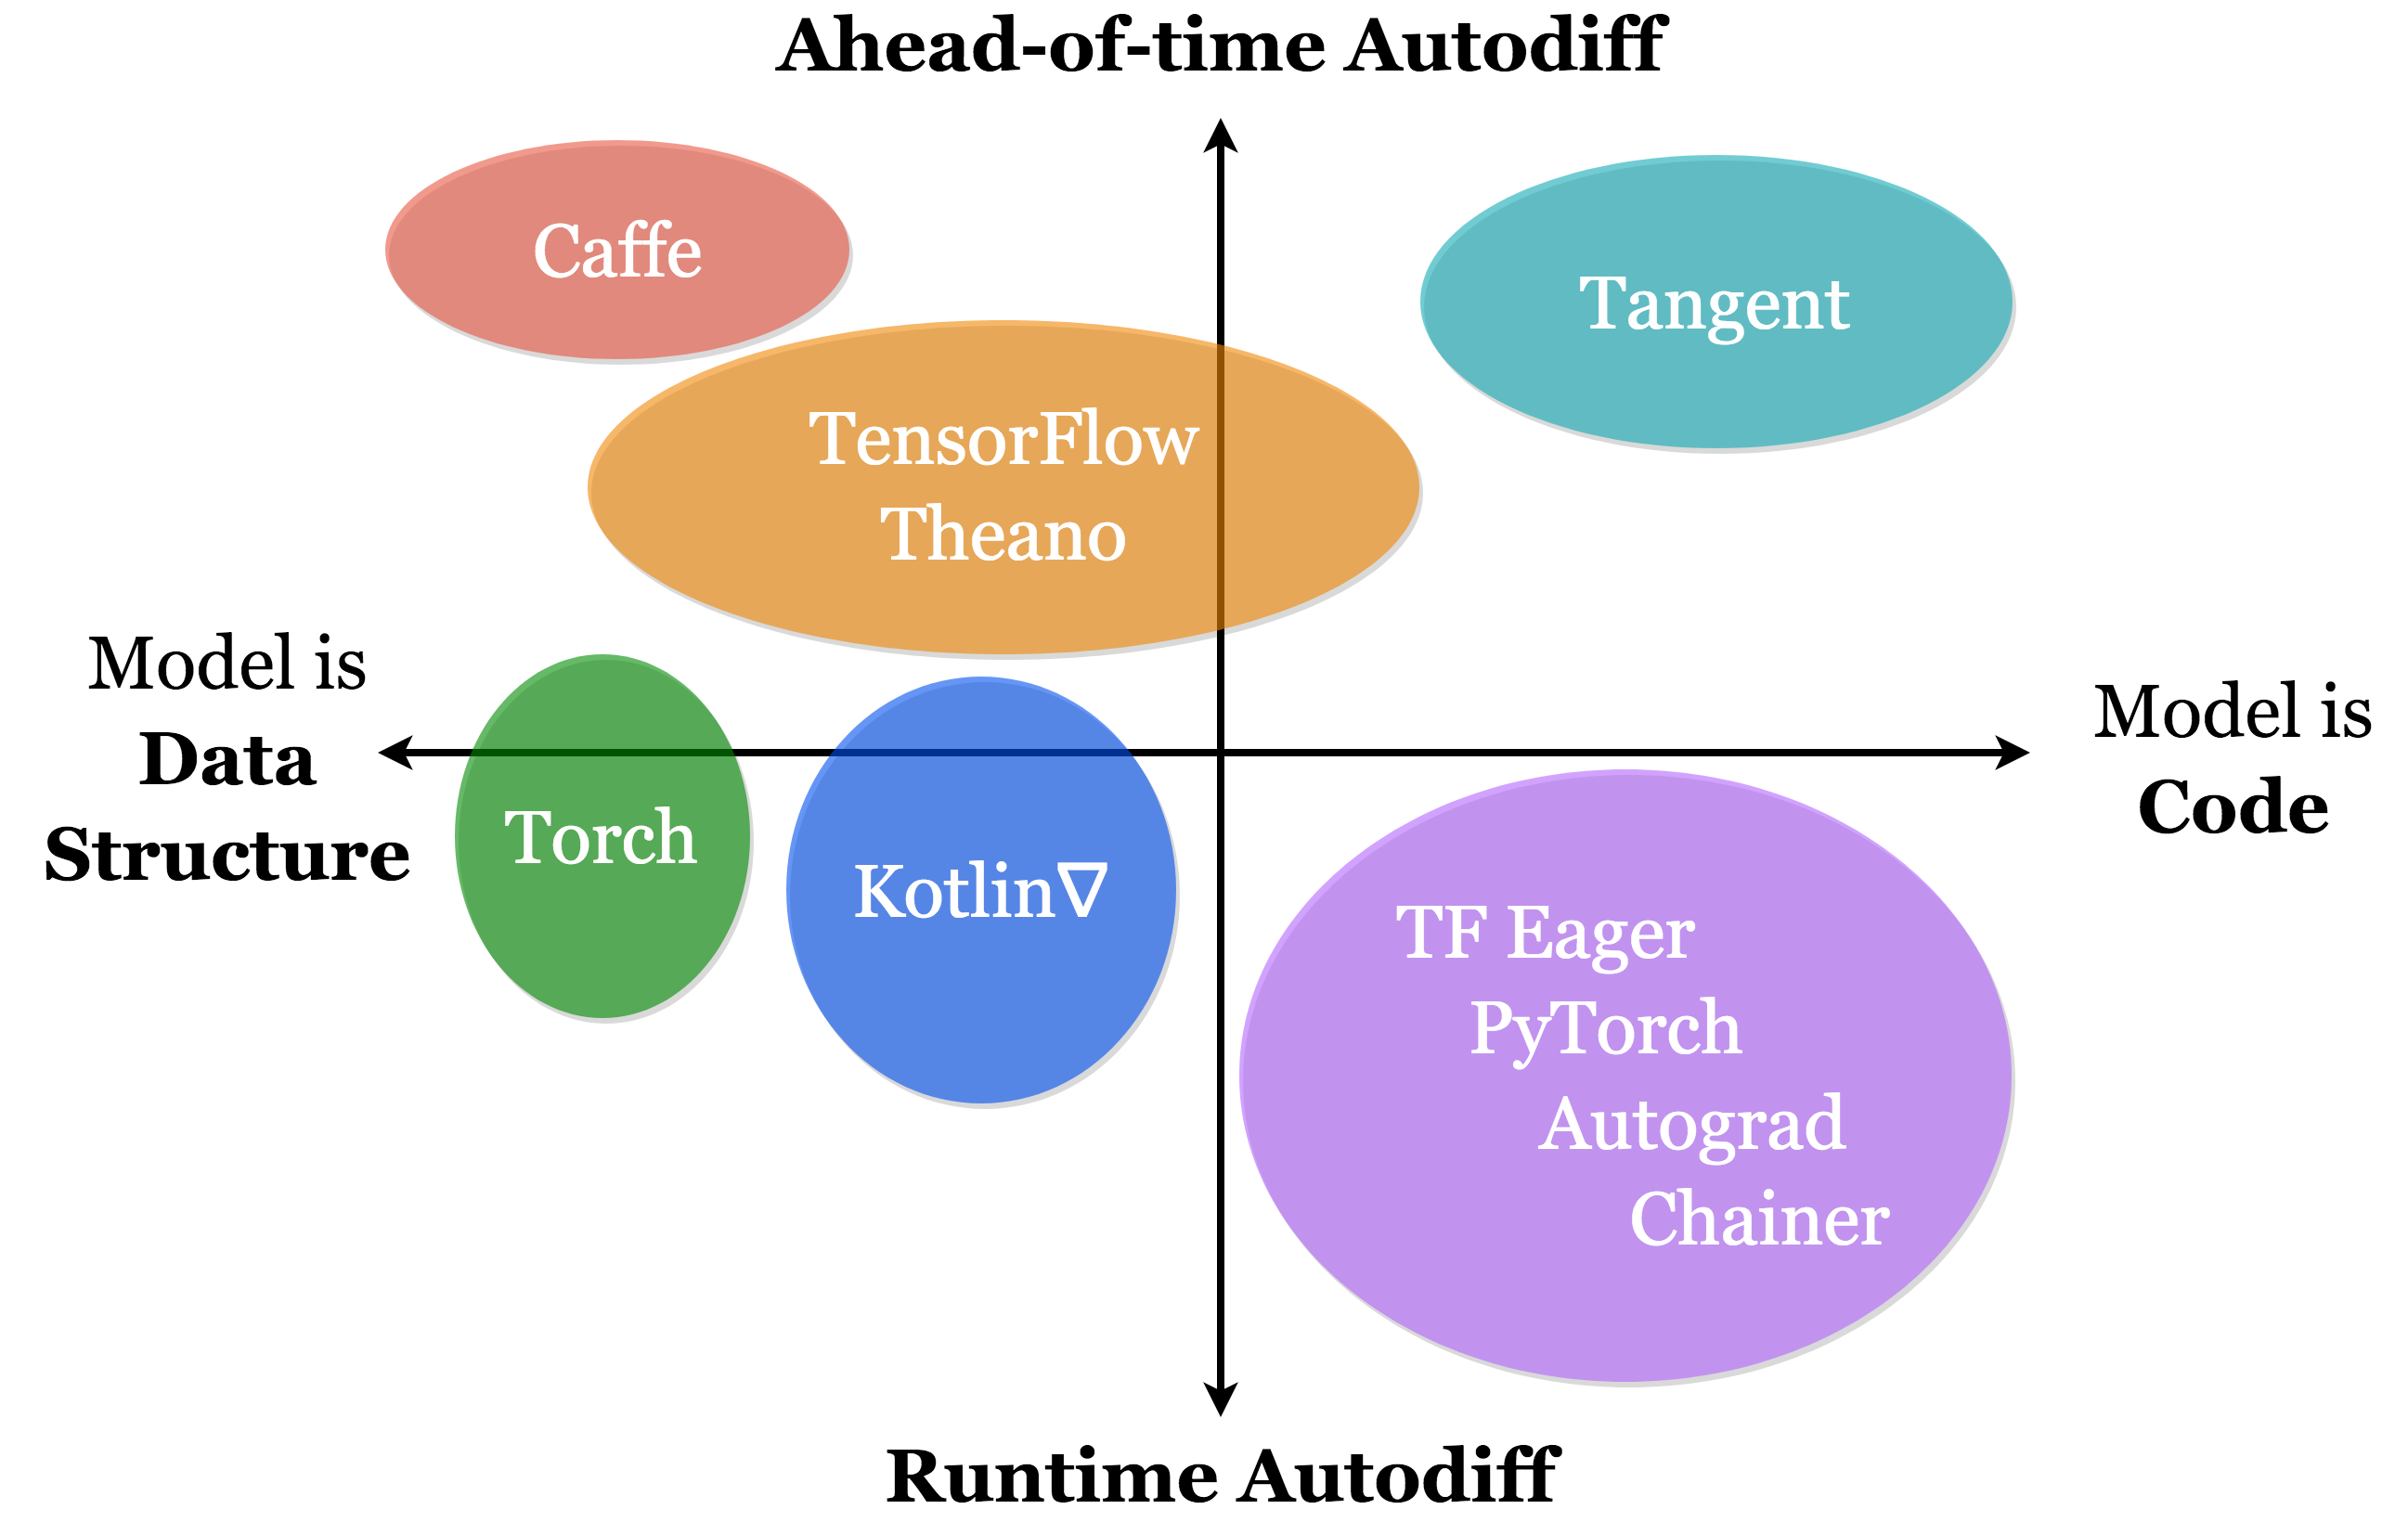
\includegraphics[width=0.70\textwidth]{kotlingrad_diagram.png}
    \caption{Adapted from~\cite{van2018tangent}. Kotlin$\nabla$ models are data structures, evaluated at runtime.}
    \label{fig:kotlingrad_digram}
\end{figure}

Kotlin$\nabla$ models are embedded domain specific languages (EDSLs), which are essentially just data structures masquerading as code. These structures may look and act like code, but are really just functions building an abstract syntax tree (AST), which can be evaluated eagerly or lazily depending on the developer's needs. Typically these ASTs represent simple state machines, but they can also be used to implement a full-fledged programming language. Popular examples include SQL/LINQ~\cite{meijer2006linq}, OptiML~\cite{sujeeth2011optiml} and other fluent interfaces~\cite{fowler05fluent}. In a sufficiently expressive host language, one can implement any language as a library, without needing to write a lexer, parser, compiler or interpreter. And with a carefully designed type system, users will automatically receive code completion and static analysis from their favorite developer tools. Many have observed that functional programming languages are suitable host languages~\cite{elliott2003compiling,rompf2010lightweight}, perhaps due to the concept of code as data and data as code\footnote{i.e.\ homoiconicity, notably introduced by Lisp, one of the first functional programming languages}.

\section{Usage}

Kotlin$\nabla$ allows users to implement differentiable programs by composing operations on numerical fields to form algebraic expressions. Expressions are lazily evaluated inside a numerical context, which may imported on a per-file basis or lexically scoped for finer-grained control over the runtime behavior.

\begin{figure}[!htb]
\begin{lstlisting}[caption={Simple code listing.}, language=Kotlin]
import edu.umontreal.kotlingrad.numerics.DoublePrecision

with(DoublePrecision) { // Use double-precision protocol
    val x = variable("x") // Declare immutable vars (these
    val y = variable("y") // are just symbolic constructs)
    val z = sin(10 * (x * x + pow(y, 2))) / 10 // Lazy exp
    val dz_dx = d(z) / d(x) // Leibniz derivative notation
    val d2z_dxdy = d(dz_dx) / d(y) // Mixed higher partial
    val d3z_d2xdy = grad(d2z_dxdy)[x] // Indexing gradient
    plot3D(d3z_d2xdy, -1.0, 1.0) // Plot in -1 < x,y,z < 1
}
\end{lstlisting}

\caption{A basic Kotlin$\nabla$ program with two inputs and one output.}
\label{label:fig1}
\end{figure}

Above, we define a function with two variables and take a series of partial derivatives with respect to each variable. The function is numerically evaluated on the interval $(-1, 1)$ in each dimension and rendered in 3-space. We can also plot higher dimensional manifolds (e.g.\ the loss surface of a neural network), projected into four dimensions, and rendered in three, where one axis is represented by time.

\begin{figure}[!htb]
    \centering $z = \sin{\big(10(x*x + y^2)\big)} / 10$, \texttt{plot}$\Big\left(\frac{\partial^{3z}}{\partial{x^2}\partial{y}}\Big\right)$ \\
    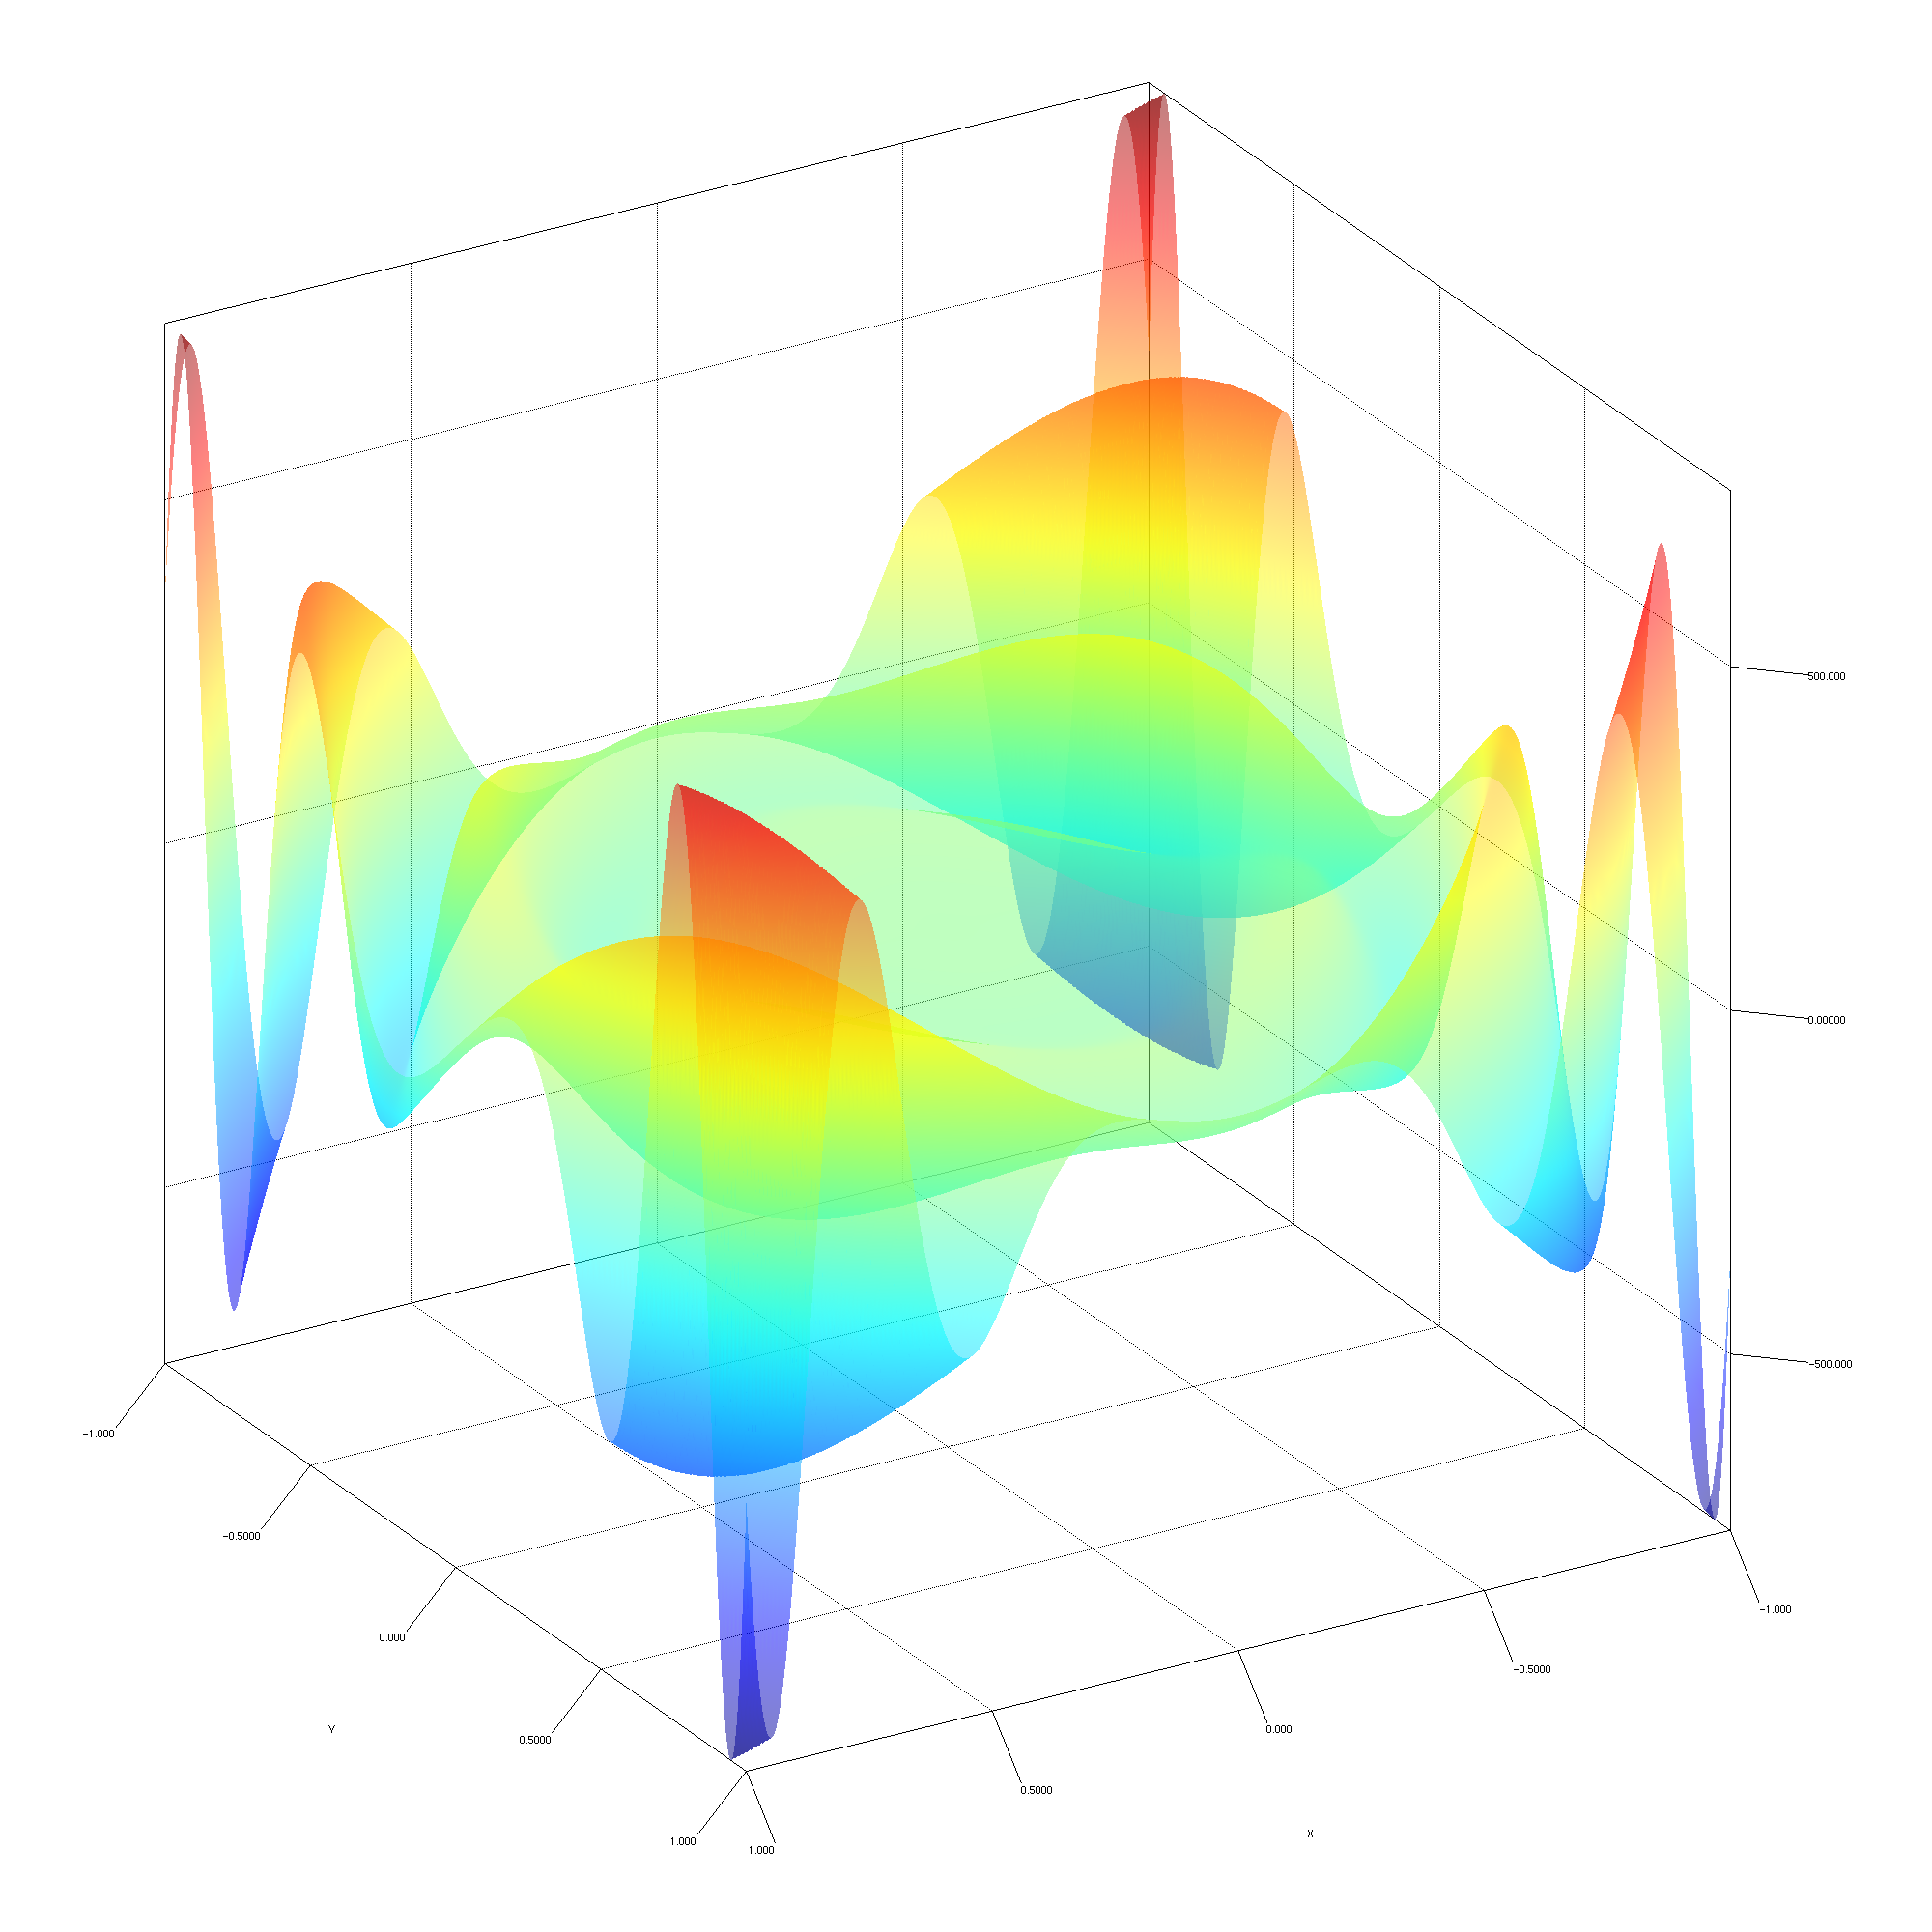
\includegraphics[scale=0.43]{plot_result.png}
    \caption{Output generated by the program shown in Figure~\ref{label:fig1}.}
\end{figure}

Kotlin$\nabla$ treats mathematical functions and programming functions with the same underlying abstraction. Expressions are composed to form a data-flow graph (DFG). An expression is simply a \texttt{Function}, which is only evaluated once invoked with numerical values, e.g. \texttt{z(0, 0)}. In this way, Kotlin$\nabla$ is similar to other compiled graph based approaches like TensorFlow and Theano.


\begin{figure}[!htb]
\begin{lstlisting}[caption={The equation below is an EDSL, and does not perform any computation.}, language=Kotlin]
val z = sin(10 * (x * x + pow(y, 2))) / 10
\end{lstlisting}
    \centering
    \begin{tikzpicture}[grow=left]
        \tikzset{level distance=45pt,sibling distance=-3pt}
        \Tree [.$\div$ [.\texttt{sin} [.$\times$ \texttt{10} [.$+$ [.$\times$ \texttt{\textbf{x}} \texttt{\textbf{x}} ] [.\texttt{pow} \texttt{\textbf{y}} \texttt{2} ] ] ] ] \texttt{10} ]
    \end{tikzpicture}
    \caption{Implicit DFG constructed by the original expression, \texttt{z}.}
\end{figure}

Kotlin$\nabla$ supports shape-safe tensor operations by encoding tensor rank as a parameter of the operand's type signature. By enumerating type-level integer literals, we can define tensor operations just once using the highest literal, and rely on Liskov substitution to preserve shape safety for subtypes.

\begin{lstlisting}[caption={Shape safe tensor addition for rank-1 tensors, $\forall L\leq2.$}, language=Kotlin]
// Literals have reified values for runtime comparison
open class `0`(override val value: Int = 0): `1`(0)
open class `1`(override val value: Int = 1): `2`(1)
class `2`(open val value: Int = 2) // Greatest literal
// <L: `2`> will accept L <= 2 via Liskov substitution
class Vec<E, L: `2`>(len: L, cts: List<E> = listOf())
// Define addition for two vectors of type Vec<Int, L>
operator fun <L: `2`, V: Vec<Int, L>> V.plus(v: V) =
Vec<Int, L>(len, cts.zip(v.cts).map { it.l + it.r })
// Type-checked vector addition with shape inference
val Y = Vec(`2`, listOf(1, 2)) + Vec(`2`, listOf(3, 4))
val X = Vec(`1`, listOf(1, 2)) + Vec(`3`) // Undefined!
\end{lstlisting}

It is possible to enforce shape-safe vector construction as well as checked vector arithmetic up to a fixed \texttt{L}, but the full implementation is omitted for brevity. A similar pattern can be applied to matrices and higher rank tensors, where the type signature encodes the shape of the operand at runtime.

With these basic ingredients, we have almost all the features necessary to build an expressive shape-safe AD, but unlike prior implementations using Scala or Haskell, in a language that is fully interoperable with Java, while also capable of compiling to JVM bytecode, JavaScript, and native code.

In future work, we intend to implement a full grammar of differentiable primitives including matrix convolution, control flow and recursion. While Kotlin$\nabla$ currently implements arithmetic manually, we plan to wrap a BLAS such as cuBLAS or native linear algebra library for performance.

\section{Type system}\label{sec:type-system}

Describing the Kotlin$\nabla$ type system (formally).

{\tiny
\begin{table}
    \begin{tabular}{|c|c|c|c|l|}
        \hline
        \multicolumn{1}{|c|}{Math}                            &  Infix                                                                         &  Prefix                                                                                 & Postfix                                                                                    & Type                                                                                                                                                                                     \\ \hline
                 $A + B$                                      & \begin{tabular}{@{}c@{}}\texttt{a + b}\\\texttt{a.plus(b)}\end{tabular}        &  \texttt{plus(a, b)}                                                                    &                                                                                            & $ (\texttt{a}:  \mathbb{R}^{\tau}\rightarrow\mathbb{R}^{\pi}, \texttt{b}: \mathbb{R}^{\lambda} \rightarrow \mathbb{R}^{\pi}) \rightarrow (\mathbb{R}^{?}\rightarrow \mathbb{R}^{\pi}) $ \\ \hline
                 $A - B$                                      & \begin{tabular}{@{}c@{}}\texttt{a - b}\\\texttt{a.minus(b)}\end{tabular}       &  \texttt{minus(a, b)}                                                                   &                                                                                            & $ (\texttt{a}:  \mathbb{R}^{\tau}\rightarrow\mathbb{R}^{\pi}, \texttt{b}: \mathbb{R}^{\lambda} \rightarrow \mathbb{R}^{\pi}) \rightarrow (\mathbb{R}^{?}\rightarrow\mathbb{R}^{\pi})  $ \\ \hline
                 $A   B$                                      & \begin{tabular}{@{}c@{}}\texttt{a * b}\\\texttt{a.times(b)}\end{tabular}       &  \texttt{times(a, b)}                                                                   &                                                                                            & $ (\texttt{a}: \mathbb{R}^{\tau}\rightarrow\mathbb{R}^{m*n}, \texttt{b}: \mathbb{R}^{\lambda}\rightarrow\mathbb{R}^{n*p})    \rightarrow (\mathbb{R}^{?}\rightarrow\mathbb{R}^{m*p})  $ \\ \hline
\begin{tabular}{@{}c@{}}$\frac{A}{B}$\\$AB^{-1}$\end{tabular} & \begin{tabular}{@{}c@{}}\texttt{a / b}\\\texttt{a.div(b)}\end{tabular}         &  \texttt{div(a, b)}                                                                     &                                                                                            & $ (\texttt{a}: \mathbb{R}^{\tau}\rightarrow\mathbb{R}^{m*n}, \texttt{b}: \mathbb{R}^{\lambda}\rightarrow\mathbb{R}^{p*n}) \rightarrow (\mathbb{R}^{?}\rightarrow\mathbb{R}^{m*p})     $ \\ \hline
\begin{tabular}{@{}c@{}}$-A$\\$+A$\end{tabular}               &                                                                                &  \begin{tabular}{@{}c@{}}\texttt{-a}\\\texttt{+a}\end{tabular}                          & \begin{tabular}{@{}c@{}}\texttt{a.unaryMinus()}\\\texttt{a.unaryPlus()}\end{tabular}       & $                   (\texttt{a}: \mathbb{R}^{\tau}\rightarrow\mathbb{R}^{\pi}) \rightarrow (\mathbb{R}^{\tau}\rightarrow\mathbb{R}^{\pi})                                             $ \\ \hline
\begin{tabular}{@{}c@{}}A+1 \\ A-1\end{tabular}               & \begin{tabular}{@{}c@{}}\texttt{a + 1}\\\texttt{a - 1}\end{tabular}            &  \begin{tabular}{@{}c@{}}\texttt{++a}\\\texttt{--a}\end{tabular}                        & \begin{tabular}{@{}c@{}}\texttt{a++, a.inc()}\\\texttt{a--, a.dec()}\end{tabular}          & $                 (\texttt{a}: \mathbb{R}^{\tau}\rightarrow\mathbb{R}^{m*m}) \rightarrow (\mathbb{R}^{\tau}\rightarrow\mathbb{R}^{m*m})                                               $ \\ \hline
\begin{tabular}{@{}c@{}}sin(a)\\cos(a)\\tan(a)\end{tabular}   &                                                                                &  \begin{tabular}{@{}c@{}}\texttt{sin(a)}\\\texttt{cos(a)}\\\texttt{tan(a)}\end{tabular} & \begin{tabular}{@{}c@{}}\texttt{a.sin()}\\\texttt{a.cos()}\\\texttt{a.tan()}\end{tabular}  & $                                            (\texttt{a}: \mathbb{R}\rightarrow\mathbb{R}) \rightarrow (\mathbb{R}\rightarrow\mathbb{R})                                              $ \\ \hline
                $\ln(A)$                                      &                                                                                &  \begin{tabular}{@{}c@{}}\texttt{ln(a)}\\\texttt{log(a)}\end{tabular}                   & \begin{tabular}{@{}c@{}}\texttt{a.ln()}\\\texttt{a.log()}\end{tabular}                     & $                  (\texttt{a}: \mathbb{R}^{\tau}\rightarrow\mathbb{R}^{m*m}) \rightarrow (\mathbb{R}^{\tau}\rightarrow\mathbb{R}^{m*m})                                              $ \\ \hline
               $\log_b A$                                     & \texttt{a.log(b)}                                                              &  \texttt{log(a, b)}                                                                     &                                                                                            & $       (\texttt{a}: \mathbb{R}^{\tau}\rightarrow\mathbb{R}^{m*m}, \texttt{b}: \mathbb{R}^{\lambda}\rightarrow\mathbb{R}^{m*m}) \rightarrow (\mathbb{R}^{?}\rightarrow\mathbb{R})     $ \\ \hline
                $A^{b}$                                       & \texttt{a.pow(b)}                                                              &  \tettt{pow(a, b)}                                                                      &                                                                                            & $       (\texttt{a}: \mathbb{R}^{\tau}\rightarrow\mathbb{R}^{m*m}, \texttt{b}: \mathbb{R}^{\lambda}\rightarrow\mathbb{R}) \rightarrow (\mathbb{R}^{?}\rightarrow\mathbb{R}^{m*m})     $ \\ \hline
\begin{tabular}{@{}c@{}}$\sqrt{a}$\\$sqrt[3](a)$\end{tabular} & \begin{tabular}{@{}c@{}}\texttt{a.pow(1.0/2)}\\\texttt{a.root(3)}\end{tabular} &  \begin{tabular}{@{}c@{}}\texttt{a.pow(1.0/2)}\\\texttt{a.root(3)}\end{tabular}         & \begin{tabular}{@{}c@{}}\texttt{a.sqrt()}\\\texttt{a.cbrt()}\end{tabular}                  & $                        (\texttt{a}: \mathbb{R}^{\tau}\rightarrow\mathbb{R}^{m*m}) \rightarrow (\mathbb{R}\rightarrow\mathbb{R}^{m*m})                                               $ \\ \hline
\begin{tabular}{@{}c@{}}$\frac{da}{db}$\\$a'(b)$\end{tabular} & \texttt{a.diff(b)}                                                             &  \texttt{grad(a)[b]}                                                                    & \texttt{d(a) / d(b)}                                                                       & $                    (\texttt{a}: C(\mathbb{R}^{m})^{*}, \texttt{b}: \mathbb{R}\rightarrow\mathbb{R}) \rightarrow (\mathbb{R}^{m}\rightarrow\mathbb{R})                               $ \\ \hline
               $\nabla a$                                     &                                                                                &  \texttt{grad(a)}                                                                       & \texttt{a.grad()}                                                                          & $                   (\texttt{a}: C(\mathbb{R}^{m})^{*}) \rightarrow (\mathbb{R}^{m}\rightarrow\mathbb{R}^{m})                                                                         $ \\ \hline
    \end{tabular}
\end{table}
}

\section{Testing}\label{sec:testing}

Kotlin$\nabla$ claims to eliminate certain runtime errors, but how do we know the proposed implementation is not incorrect? One method, borrowed from the Haskell community, is called property-based testing (PBT), closely related to metamorphic testing. Notable implementations include QuickCheck, Hypothesis and ScalaTest (ported to Kotlin in KotlinTest). PBT uses algebraic properties to verify the result of an operation by constructing semantically equivalent but syntactically distinct expressions, which should produce the same answer. Kotlin$\nabla$ uses two such equivalences to validate its AD implementation:

\begin{enumerate}
    \item \textbf{Symbolic differentiation}: manually differentiate and compare the values returned on a subset of the domain with AD.
    \item \textbf{Finite difference approximation}: sample space of symbolic (differentiable) functions, comparing results of AD to FD.
\end{enumerate}

\noindent For example, the following test checks whether the manual derivative and the automatic derivative, when evaluated at a given point, are equal to within numerical precision:

\begin{lstlisting}[language=Kotlin, showstringspaces=false]
val x = Var("x")
val y = Var("y")
val z = y * (sin(x * y) - x)            // Function under test
val dz_dx = d(z) / d(x)                 // Automatic derivative
val manualDx = y * (cos(x * y) * y - 1) // Manual derivative

"dz/dx should be y * (cos(x * y) * y - 1)" {
    NumericalGenerator.assertAll { x0, y0 ->
        // Evaluate the results at a given seed
        val autoEval = dz_dx(x to x0, y to y0)
        val manualEval = manualDx(x to x0, y to y0)
        // Should pass iff |adEval - manualEval| < eps
        autoEval shouldBeApproximately manualEval
    }
}
\end{lstlisting}

PBT will search the input space for two numerical values \texttt{x0} and \texttt{y0}, which violate the specification, then "shrink" them to discover pass-fail boundary values. We can construct a similar test using finite differences:

\begin{lstlisting}[language=Kotlin, showstringspaces=false]
"d(sin x)/dx should be equal to (sin(x + dx) - sin(x)) / dx" {
    NumericalGenerator.assertAll { x0 ->
        val f = sin(x)
        val df_dx = d(f) / d(x)
        val adEval = df_dx(x0)
        val dx = 1E-8
        val fdEval = (sin(x0 + dx) - sin(x0)) / dx
        adEval shouldBeApproximately fdEval
    }
}
\end{lstlisting}

There are many other ways to independently verify the numerical gradient, such as dual numbers or the complex step derivative. Another method is to compare the numerical output against a well-known implementation, such as TensorFlow. We plan to conduct a more thorough comparison of numerical accuracy and performance.

\section{Shape safety}\label{sec:shape-safety}

\noindent There are three broad strategies for handling shape errors in numerical programming: \\

\begin{enumerate}
    \item Hide the error somehow by implicitly reshaping or broadcasting arrays
    \item Announce the error at runtime, with a relevant message, e.g.~\texttt{InvalidArgumentError}
    \item Do not allow programs which can result in a shape error to compile \\
\end{enumerate}

\noindent In Kotlin$\nabla$, we use the third strategy. Consider the following program:

\begin{lstlisting}[language=Kotlin]
// Inferred type: Vec<Int, `2`>
val a = Vec(1.0, 2.0)
// Inferred type: Vec<Int, `3`>
val b = Vec(1.0, 2.0, 3.0)
val c = b + b
// Does not compile, shape mismatch
// a + b
\end{lstlisting}

\noindent Attempting to sum two vectors whose shapes do not match will fail to compile:

\begin{lstlisting}[language=Kotlin]
// Inferred type: Mat<Double, `1`, `4`>
val a = Mat(`1`, `4`, 1.0, 2.0, 3.0, 4.0)
// Inferred type: Mat<Double, `4`, `1`>
val b = Mat(`4`, `1`, 1.0, 2.0, 3.0, 4.0)
val c = a * b
// Does not compile, inner dimension mismatch
// a * a
// b * b
\end{lstlisting}

\noindent Similarly, multiplying two tensors whose inner dimensions do not match will not compile:

\begin{lstlisting}[language=Kotlin]
val a = Mat(`2`, `4`,
    1.0, 2.0, 3.0, 4.0,
    5.0, 6.0, 7.0, 8.0
)
val b = Mat(`4`, `2`,
    1.0, 2.0,
    3.0, 4.0,
    5.0, 6.0,
    7.0, 8.0
)
// Types are optional, but encouraged
val c: Mat<Double, `2`, `2`> = a * b
val d = Mat(`2`, `1`, 1.0, 2.0)
val e = c * d
val f = Mat(`3`, `1`, 1.0, 2.0, 3.0)
// Does not compile, inner dimension mismatch
// e * f
\end{lstlisting}

Explicit types are optional but encouraged. Type inference helps preserve shape information over long programs.

\begin{lstlisting}[language=Kotlin]
fun someMatFun(m: Mat<Double, `3`, `1`>): Mat<Double, `3`, `3`> = ...
fun someMatFun(m: Mat<Double, `2`, `2`>) = ...
\end{lstlisting}

When writing a function, it is mandatory to declare the input type(s), but the return type may be omitted. Shape-safety is currently supported up to rank-2 tensors, i.e.\ matrices.

While first-class dependent types are useful for ensuring arbitrary shape safety (e.g.\ when concatenating and reshaping matrices), they are unnecessary for simple equality checking (such as when multiplying two matrices)\footnote{Many less powerful type systems are still capable of performing arbitrary computation in the type checker. As specified, Java's type system is known to be Turing Complete. It may be possible to emulate a limited form of dependent types in Java by exploiting this property, although this may not computationally tractable due to the practical limitations noted by Grigore~\cite{Grigore:2017:JGT:3009837.3009871}.}. When the shape of a tensor is known at compile time, it is possible to encode this information using a less powerful type system, as long as it supports subtyping and parametric polymorphism. In practice, we can implement a shape-checked tensor arithmetic in languages like Java, Kotlin, C++, C\# or Typescript, which accept generic type parameters. In Kotlin, whose type system is less expressive than Java, we use the following strategy.

First, we enumerate a list of integer type literals as a chain of subtypes, so that \texttt{0 <: 1 <: 2 <: 3 <: ... <: C}, where \texttt{C} is the largest fixed-length dimension we wish to represent. Using this encoding, we are guaranteed linear growth in space and time for subtype checking. C can be specified by the user, but they will need to rebuild this project from scratch.

\begin{lstlisting}[language=Kotlin]
open class `0`(override val i: Int = 0): `1`(i) { companion object: `0`(), Nat<`0`> }
open class `1`(override val i: Int = 1): `2`(i) { companion object: `1`(), Nat<`1`> }
open class `2`(override val i: Int = 2): `3`(i) { companion object: `2`(), Nat<`2`> }
open class `3`(override val i: Int = 3): `4`(i) { companion object: `3`(), Nat<`3`> }
//...This is generated
sealed class `100`(open val i: Int = 100) { companion object: `100`(), Nat<`100`> }
interface Nat<T: `100`> { val i: Int } // Used for certain type bounds
\end{lstlisting}

Kotlin$\nabla$ supports shape-safe tensor operations by encoding tensor rank as a parameter of the operand’s type signature. Since integer literals are a chain of subtypes, we need only define tensor operations once using the highest literal, and can rely on Liskov substitution to preserve shape safety for all subtypes. Let us consider the rank-1 tensor (i.e.\ vector) case:

\begin{lstlisting}[language=Kotlin]
infix operator fun <C: `100`, V: Vec<Float, C>> V.plus(v: V): Vec<Float, C> =
    Vec(length, contents.zip(v.contents).map { it.first + it.second })
\end{lstlisting}

\noindent This technique can be easily extended to additional infix operators. We can also define a shape-safe vector initializer by overloading the invoke operator on a companion object:

\begin{lstlisting}[language=Kotlin]
open class Vec<E, MaxLength: `100`> constructor(
    val length: Nat<MaxLength>,
    val contents: List<E> = listOf()
) {
    operator fun get(i: `100`): E = contents[i.i]
    operator fun get(i: Int): E = contents[i]
    companion object {
        operator fun <T> invoke(t: T): Vec<T, `1`> = Vec(`1`, listOf(t))
        operator fun <T> invoke(t0: T, t1: T): Vec<T, `2`> = Vec(`2`, listOf(t0, t1))
        operator fun <T> invoke(t0: T, t1: T, t2: T): Vec<T, `3`> = Vec(`3`, listOf(t0, t1, t2))
        //...
    }
}
\end{lstlisting}

The initializer may be omitted in favor of dynamic construction, although this may fail at runtime. For example:

\begin{lstlisting}[language=Kotlin]
val one = Vec(`3`, 1, 2, 3) + Vec(`3`, 1, 2, 3)   // Always runs safely
val add = Vec(`3`, 1, 2, 3) + Vec(`3`, listOf(t)) // May fail at runtime
val vec = Vec(`2`, 1, 2, 3)                       // Does not compile
val sum = Vec(`2`, 1, 2) + add                    // Does not compile
\end{lstlisting}

A similar syntax is possible for matrices and higher-rank tensors. For example, Kotlin$\nabla$ can infer the shape of multiplying two matrices, and will not compile if their inner dimensions do not match:

\begin{lstlisting}[language=Kotlin]
// Inferred type: Mat<Int, `4`, `4`>
val l = Mat(`4`, `4`,
    1, 2, 3, 4,
    5, 6, 7, 8,
    9, 0, 0, 0,
    9, 0, 0, 0
)
// Inferred type: Mat<Int, `4`, `3`>
val m = Mat(`4`, `3`,
    1, 1, 1,
    2, 2, 2,
    3, 3, 3,
    4, 4, 4
)

// Inferred type: Mat<Int, `4`, `3`>
val lm = l * m
// m * m // Does not compile
\end{lstlisting}

A similar technique is possible in Haskell, which is capable of a more powerful form of type-level computation \textit{type arithmetic}. Type arithmetic makes it easy to express convolutional arithmetic and other arithmetic operations on shape variables (say, splitting a vector in half), which is currently not possible, or would require enumerating every possible combination of type literals.

\section{Operator overloading}\label{sec:operator-overloading}

Operator overloading enables concise notation for arithmetic on abstract types, where the types encode algebraic structures, e.g. \texttt{Group}, \texttt{Ring}, and \texttt{Field}. These abstractions are extensible to other kinds of mathematical structures, such as complex numbers and quaternions.

For example, suppose we have an interface \texttt{Group}, which overloads the operators $+$ and $\times$, and is defined like so:

\begin{lstlisting}[caption={Simple code listing.}, language=Kotlin]
interface Group<T: Group<T>> {
    operator fun plus(addend: T): T
    operator fun times(multiplicand: T): T
}
\end{lstlisting}

Here, we specify a recursive type bound using a method known as F-bounded polymorphism~\cite{canning1989f} to ensure that operations return the concrete type variable T, rather than something more generic like \texttt{Group} (effectively, \texttt{T} is a \texttt{self} type). Imagine a class \texttt{Expr} which has implemented \texttt{Group}. It can be used as follows:

\begin{lstlisting}[caption={Simple code listing.}, language=Kotlin]
fun <T: Group<T>> cubed(t: T): T = t * t * t
fun <E: Expr<E>> twiceExprCubed(e: E): E = cubed(e) + cubed(e)
\end{lstlisting}

Like Python, Kotlin supports overloading a limited set of operators, which are evaluated using a fixed precedence. In the current version of Kotlin$\nabla$, operators do not perform any computation, they simply construct a directed acyclic graph representing the symbolic expression. Expressions are only evaluated when invoked as a function.

\section{First-class functions}\label{sec:first-class-functions}

With higher-order functions and lambdas, Kotlin treats functions as first-class citizens. This allows us to represent mathematical functions and programming functions with the same underlying abstractions (typed FP). A number of recent papers have demonstrated the expressiveness of this paradigm for automatic differentiation.

In Kotlin$\nabla$, all expressions can be treated as functions. For example:

\begin{lstlisting}[caption={Simple code listing.}, language=Kotlin]
fun <T: Group<T>> makePoly(x: Var<T>, y: Var<T>) = x * y + y * y + x * x

val x: Var<Double> = Var(1.0)
val f = makePoly(x, y)
val z = f(1.0, 2.0) // Returns a value
println(z) // Prints: 7
\end{lstlisting}

Currently, it is only possible to represent functions where all inputs and outputs share a single type. In future iterations, it is possible to extend support for building functions with varying input/output types and enforce constraints on both, using covariant and contravariant type bounds.

\section{Coroutines}\label{sec:coroutines}

Coroutines are a generalization of subroutines for non-preemptive multitasking, typically implemented using continuations. One form of continuation, known as shift-reset a.k.a.\ delimited continuations, are sufficient for implementing reverse mode AD with operator overloading alone (without any additional data structures) as described by Wang et al. in Shift/Reset the Penultimate Backpropagator~\cite{wang2018demystifying} and later in Backpropagation with Continuation Callbacks~\cite{wang2018backpropagation}. Delimited continuations can be implemented using Kotlin coroutines and they are currently a work in progress.

\section{Extension Functions}\label{sec:extension-functions}

Extension functions augment external classes with new fields and methods. Via context oriented programming, Kotlin$\nabla$ can expose its custom extensions (e.g.\ in \texttt{DoublePrecision}) to consumers without requiring subclasses or inheritance.

\begin{lstlisting}[caption={Using extension functions we can provide numerical conversions for common data types, wrapped by a Context.}, language=Kotlin]
data class Const<T: Group<T>>(val number: Double) : Expr()
data class Sum<T: Group<T>>(val e1: Expr, val e2: Expr) : Expr()
data class Prod<T: Group<T>>(val e1: Expr, val e2: Expr) : Expr()

class Expr<T: Group<T>>: Group<Expr<T>> {
    operator fun plus(addend: Expr<T>) = Sum(this, addend)
    operator fun times(multiplicand: Expr<T>) = Prod(this, multiplicand)
}

object DoubleContext {
    operator fun Number.times(expr: Expr<Double>) = Const(toDouble()) * expr
}
\end{lstlisting}

Now, we can use the context to define another extension, Expr.multiplyByTwo, which computes the product inside a DoubleContext, using the operator overload we defined above:

\begin{lstlisting}[caption={Simple code listing.}, language=Kotlin]
fun Expr<Double>.multiplyByTwo() = with(DoubleContext) { 2 * this }
\end{lstlisting}

Extensions can also be defined in another file or context and imported on demand. This approach was borrowed from KMath~\cite{nozik2019acat}, another mathematical library for Kotlin.

\section{Algebraic data types}\label{sec:adts}

Algebraic data types (ADTs) in the form of sealed classes (a.k.a.\ sum types) allows creating a closed set of internal subclasses to guarantee an exhaustive control flow over the concrete types of an abstract class. At runtime, we can branch on the concrete type of the abstract class. For example, suppose we have the following classes:

\begin{lstlisting}[caption={Users must handle all subclasses when branching on the type of a sealed class, as incomplete control flow will not compile (instead of failing silently at runtime).}, language=Kotlin]
sealed class Expr<T: Group<T>>: Group<Expr<T>> {
    fun diff() = when(expr) {
       is Const -> Zero
       // Smart casting allows us to access members of a checked typed without explicit casting
       is Sum -> e1.diff() + e2.diff()
       // Product rule: d(u*v)/dx = du/dx * v + u * dv/dx
       is Prod -> e1.diff() * e2 + e1 * e2.diff()
       is Var -> One
       // Since the subclasses of Expr are a closed set, no `else -> ...` is required.
    }

    operator fun plus(addend: Expr<T>) = Sum(this, addend)
    operator fun times(multiplicand: Expr<T>) = Prod(this, multiplicand)
}

data class Const<T: Group<T>>(val number: Double) : Expr()
data class Sum<T: Group<T>>(val e1: Expr, val e2: Expr) : Expr()
data class Prod<T: Group<T>>(val e1: Expr, val e2: Expr) : Expr()
class Var<T: Group<T>>: Expr()
class Zero<T: Group<T>>: Const<T>
class One<T: Group<T>>: Const<T>
\end{lstlisting}

Smart-casting allows us to treat the abstract type Expr as a concrete type, e.g. Sum after performing an is Sum check. Otherwise, we would need to write (expr as Sum).e1 in order to access its field, e1. Performing a cast without checking would throw a runtime exception, if the type were incorrect. Using sealed classes helps avoid casting, thus avoiding ClassCastExceptions.

\section{Multiple Dispatch}\label{sec:multiple-dispatch}

In conjunction with ADTs, Kotlin$\nabla$ also uses multiple dispatch to instantiate the most specific result type of applying an operator based on the type of its operands. While multiple dispatch is not an explicit language feature, it can be emulated using inheritance.

Building on the previous example, a common task in AD is to simplify a graph. This is useful in order to minimize the number of calculations required, or to improve numerical stability. We can eagerly simplify expressions based on algebraic rules of replacement. Smart casting allows us to access members of a class after checking its type, without explicitly casting it:

\begin{lstlisting}[caption={Multiple dispatch allows us to put all related control flow on a single abstract class which is inherited by subclasses, simplifying readability, debugging and refactoring.}, language=Kotlin]
override fun times(multiplicand: Function<X>): Function<X> =
    when {
        this == zero -> this
        this == one -> multiplicand
        multiplicand == one -> this
        multiplicand == zero -> multiplicand
        this == multiplicand -> pow(two)
        this is Const && multiplicand is Const -> const(value * multiplicand.value)
        // Further simplification is possible using rules of replacement
        else -> Prod(this, multiplicand)
    }

val result = Const(2.0) * Sum(Var(2.0), Const(3.0))
//         = Sum(Prod(Const(2.0), Var(2.0)), Const(6.0))
\end{lstlisting}

\section{Numeric Tower}\label{sec:numeric-tower}

Kotlin$\nabla$ uses a numeric tower~\cite{st2012typing}. First pioneered in Scheme\cite{sperber2009revised}, this strategy is well-suited to object oriented programming~\cite{niculescu2003design, niculescu2011using} and is widely used in other mathematical libraries such as KMath~\cite{nozik2019acat} and Apache Commons Math~\cite{developers2012apache}. By doing so, we are able to define common functionality on the supertype.

\begin{lstlisting}[caption={Many common mathematical operations can be defined in simpler terms.}, language=Kotlin]
interface Field<X: Field<X>> {
    val e: X
    val one: X
    val zero: X
    operator fun unaryMinus(): X
    operator fun plus(addend: X): X
    operator fun minus(subtrahend: X): X = this + -subtrahend
    operator fun times(multiplicand: X): X
    operator fun div(dividend: X): X = this * dividend.pow(-one)
    infix fun pow(exp: X): X
    fun ln(): X
}
\end{lstlisting}

Furthermore, if we need to later define a field over the quaternions (suppose for backpropogating through a quaternion neural network~\cite{isokawa2003quaternion}), these abstractions are easy to extend, since we only need to implement a very small set of primitive operations.

\section{Comparison}\label{sec:comparison}

\begin{center}
\begin{tabular}{llllllll}
    Framework &
    Language &
    \rot{Automatic Differentiation} &
    \rot{Functional Programming} &
    \rot{Type Safe} &
    \rot{Shape Safe} &
    \rot{Differentiable Programming} &
    \rot{Multiplatform}
    \\ \hline
Kotlin$\nabla$                                                                 & Kotlin   & \cmark & \cmark                                                 & \cmark                                                 & \cmark                                         & \wmark                                                     & \wmark                                                     \\
DiffSharp                   & F\#      & \cmark & \cmark                                                 & \cmark                                                 & \xmark                                                          & \cmark                                               & \xmark                                                                \\
TensorFlow.FSharp & F\#      & \cmark & \cmark                                                 & \cmark                                                 & \cmark                                         & \cmark                                               & \xmark                                                                \\
Myia                            & Python   & \cmark & \cmark                                                 & \cmark                                                 & \cmark                                         & \cmark                                               & \xmark                                                                \\
Deeplearning.scala      & Scala    & \cmark & \cmark                                                 & \cmark                                                 & \xmark                                                          & \cmark                                               & \xmark                                                                \\
Nexus                                    & Scala    & \cmark & \cmark                                                 & \cmark                                                 & \cmark                                         & \cmark                                               & \xmark                                                                \\
Lantern                    & Scala    & \cmark & \cmark                                                 & \cmark                                                 & \xmark                                                          & \cmark                                               & \xmark                                                                \\
Grenade                    & Haskell  & \cmark & \cmark                                                 & \cmark                                                 & \cmark                                         & \xmark                                                                & \xmark                                                                \\
Eclipse DL4J                          & Java     & \cmark & \xmark                                                                  & \cmark                                                 & \xmark                                                          & \xmark                                                                & \xmark                                                                \\
Halide                                    & C++      & \cmark & \xmark                                                                  & \cmark                                                 & \xmark                                                          & \cmark                                               & \xmark                                                                \\
Stalin$\naba$         & Scheme   & \cmark & \cmark & \xmark & \xmark & \xmark & \xmark \\
\end{tabular}
\end{center}

\rare{\chapter{Verification and validation}\label{ch:difftest}}

\setlength{\epigraphwidth}{0.78\textwidth}
\epigraph{``If we use, to achieve our purposes, a mechanical agency with whose operation we cannot efficiently interfere\ldots then we had better be quite sure the purpose put into the machine is the purpose which we really desire.''}{\begin{flushright}--Norbert Weiner, \textit{Some moral and technical consequences of automation}~\cite{wiener1960some}\end{flushright}}

\section{Adversarial test case generation}

Neural networks and differentiable programming has provided a powerful new set of optimization tools for training learning algorithms. However these methods are often brittle to small variations in the input space, and have difficulty with generalization. In contrast, these same techniques used for probing the failure modes of neural networks can be applied to adversarial test case generation for traditional programs.

\section{Background}

Suppose we have a program $P: \mathbb{R}\rightarrow\mathbb{R}$ where:
%
\begin{equation}
    P(x)=p_n \circ p_{n-1} \circ p_{n-2} \circ ... \circ p_1 \circ p_0
\end{equation}
%
From the chain rule of calculus, we know that:
%
\begin{equation}
    \frac{dP}{dp_0} = {\displaystyle \prod_{i=1}^{n} \frac{dp_{i}}{dp_{i-1}}}
\end{equation}

%
% Imagine a set of tests $\mathrm{T}: \mathbb{R} \rightarrow \mathbb{B}$ where $\mathrm{T}={\tau_1, ...\tau_m}$.  For example,
%
Imagine a single test $T: \mathbb{R} \rightarrow \mathbb{B}$. Consider the following example::
%
\begin{equation}
    T: \forall x \in (0, 1), P(x) < C
\end{equation}
%
How can we find a set of inputs that break the test under a fixed computational budget (i.e.\ constant number of program evaluations)? In other words:
%
\begin{equation}
    D_T: \{ x^i \sim \mathbb{R}(0, 1) \mid P(x^i) \implies \neg T \}, maximize |D_T|
\end{equation}
%

If we have no information about the program implementation or its input distribution, $D_P$, we can do no better than random search~\cite{wolpert1997no}. However, if we know something about the input distribution, we could re-parameterize the distribution to incorporate our knowledge. Assuming the program has been tested on common inputs, we might consider sampling $x \sim \frac{1}{D_P}$ for inputs that are infrequent. If we knew how $P$ were implemented, we could prioritize our search in input regions leading towards internal discontinuities (e.g.\ edge cases in software testing). However for functions that are continuous and differentiable, these heuristics are almost certainly insufficient.

% Finally, we could train a neural network to predict inputs that were likely to cause a program to fail a given specification. As input, the network would take the function and test cases, and as its output, produce values that were likely to violate $T$.

Another strategy, independent of how candidate inputs are selected, is to use some form of gradient based optimization in the search procedure. For example in (3) we could have a loss function:
%
\begin{equation}
    \mathcal{L}(P, x) = C - P(x)
\end{equation}
%
The gradient of the loss w.r.t. $x$ (assuming $P$ is fixed\footnote{In contrast with backpropogation, where the parameters are updated.}) is:
%
\begin{equation}
    \nabla \mathcal{L}(P, x) = - \frac{dP}{dx}
\end{equation}
%
Where the vanilla gradient update step is defined as:
%
\begin{equation}
    x_{n+1}^i=x_{n}^i - \alpha\frac{dP}{dx}
\end{equation}
%
We hypothesize that if the implementation of $P$ were flawed and a counterexample to (3) existed, as sample size increased, a subset of gradient descent trajectories would fail to converge, a portion would converge to local minima, and a subset of trajectories would discover inputs violating the program specification. How would such a search procedure look in practice? Consider the following algorithm:

% Furthermore, we hypothesize that if a sufficiently large fraction of the input space existed where $T$ were false, then as we sample from that space, the probability of detection would approach 1:
%
% \begin{equation}
%     (\forall i \in I^\dagger, p(i) \implies \neg T) \implies \lim_{|x|\to \infty}Prob(\hat{T}=False) = 1
% \end{equation}
%

%\begin{algorithm}
%    \SetKwInOut{Input}{Input}
%    \SetKwInOut{Output}{Output}
%
%    \Input{Program $P$, specification $T$, evaluation budget $Budget$}
%    \Output{$D_T$, the set of inputs which cause $P$ to fail on T}
%    $D_T$ = []\;
%    evalCount = 0\;
%    \While{evalCount \leq $Budget$} {
%    sample candidate input $x^i$ according to selection strategy S\;
%    \eIf{$P(x^i)\implies$ \neg T}{
%    append $x^i$ to D_T\;
%
%    }{
%    n = 0\;
%    $x^i_n = x^i$\;
%
%    \While{$n \leq C \land evalCount \leq Budget$ \land $\neg converged$} {
%    n++\;
%
%    $x_{n}^i=x_{n-1}^i - \alpha\frac{dP}{dx}$\;
%
%
%    \If{P(x^i_n) \implies T} {
%    append $x^i_n$ to D_T\;
%
%    break\;
%
%    }
%
%    evalCount++\;
%    }
%    }
%    evalCount++; i++\;
%    }
%
%    \caption{Algorithm for finding test failures. First select a candidate input $x^i$ according to sampling strategy $S$ (e.g.\ uniform random, or a neural network which takes $P$ and $T$ as input). If $P(x^i)$ violates $T$, we can append $x^i$ to $D_T$ and repeat. Otherwise, we follow the gradient of $\mathcal{L}(P, x)$ with respect to $x$ and repeat until test failure, gradient descent convergence, or a fixed number of steps $C$ are reached before resampling $x^{i+1}$ from the initial sampling strategy $S$ to ensure each gradient descent trajectory will terminate before exhausting our budget.}
%\end{algorithm}

\section{Regression testing and forgetting}

An endemic problem in modern deep learning is the problem of forgetting. In order to combat this issue, we turn to a classic software testing tool: regression testing.

Regular regression testing gives clear diagnostics about the behavior of intelligent systems.

\mediumrare{\chapter{Software Maitenance and Reproducibility}\label{ch:software-reproducibility}}

In this chapter, we will discuss the challenges of software reproducibility and how best practices in software engineering like continuous integration and delivery can help researchers mitigate the variability associated with building and running software. Docker~\cite{merkel2014docker} is one technical solution we will discuss. Our work is roughly related to computational determinism, and does not consider the variability of distributional shift or related statistical notions of variation.

\section{Operating systems and virtualization}\label{sec:os-and-virtualization}

In 2006, Linux began introducing a variety of new kernel features for controlling groups of processes, under the aegis of \textbf{cgroups}~\cite{menage2007adding}. Collectively, these features supported a kind of lightweight virtualization, where a fully virtual machine was no longer necessary to get many of the benefits of VMs, primarily resource control and namespace isolation. These features paved the way for a set of tools that are today known as containers. Unlike VMs, containers share a common kernel, but remain isolated from the host OS and sibling containers. While the overhead of running VMs often limits their deployment to server-class hardware, container's are comparatively lightweight, which enables them to run on a far broader class of mobile and embedded platforms.

\section{Dependency management}\label{sec:dependency-management}

One common source of software variability are dependencies and the dependency solving problem. In fact, operating systems have struggled with this issue for a number of years before it was realized that dependency resolution was NP-complete~\cite{abate2012dependency}.

\section{Containerization}\label{sec:containerization}

One of the challenges of distributed software development across heterogeneous platforms is the problem of variability. With the increasing pace of software development comes the added burden of software maintenance. As hardware and software stacks evolve, so too must source code be updated to build and run correctly. Maintaining a stable and well documented codebase can be a considerable challenge, especially in a robotics setting where contributors are frequently joining and leaving the project. Together, these challenges present significant obstacles to experimental reproducibility and scientific collaboration.

In order to address the issue of software reproducibility, we developed a set of tools and development workflows that draw on best practices in software engineering. These tools are primarily built around containerization, a widely adopted virtualization technology in the software industry. In order to lower the barrier of entry for participants and minimize variability across platforms (e.g.\ simulators, robotariums, Duckiebots), we provide a state-of-the-art container infrastructure based on Docker, a popular container engine. Docker allows us to construct versioned deployment artifacts that represent the entire filesystem and to manage resource constraints via a sandboxed runtime environment.

\begin{figure}[ht]
    \centering
    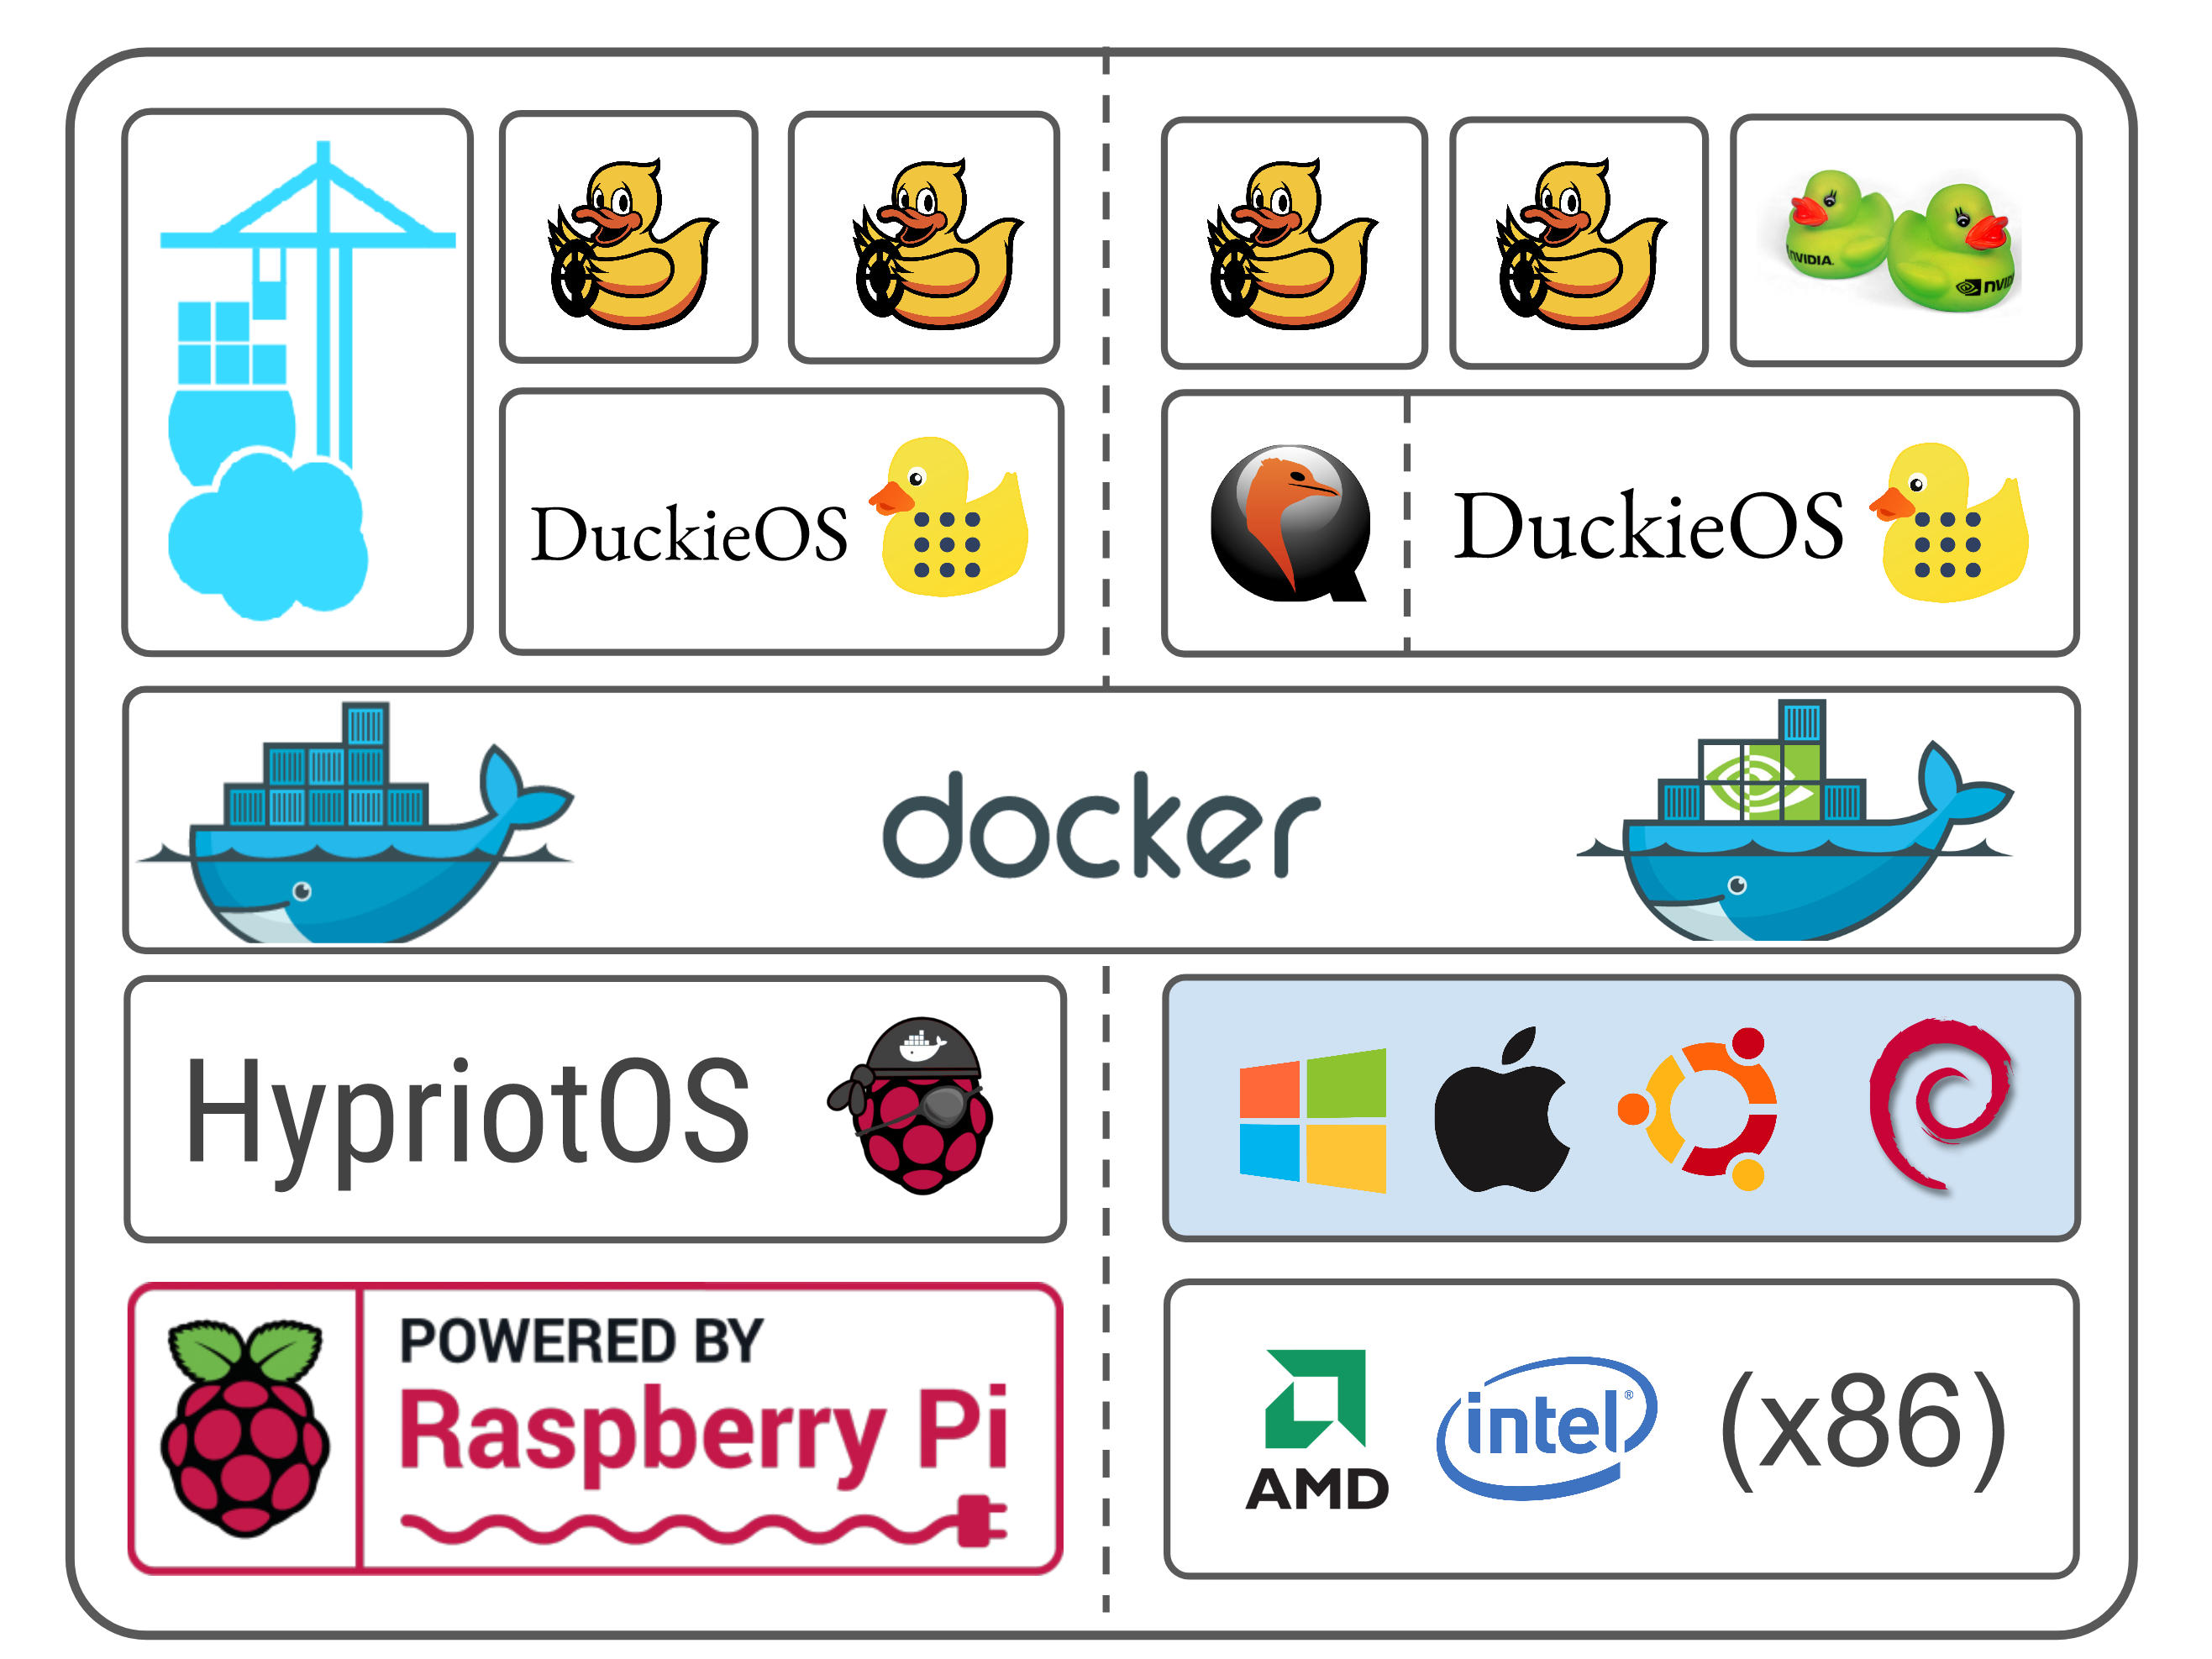
\includegraphics[width=0.45\textwidth]{docker_stack_1.png}
    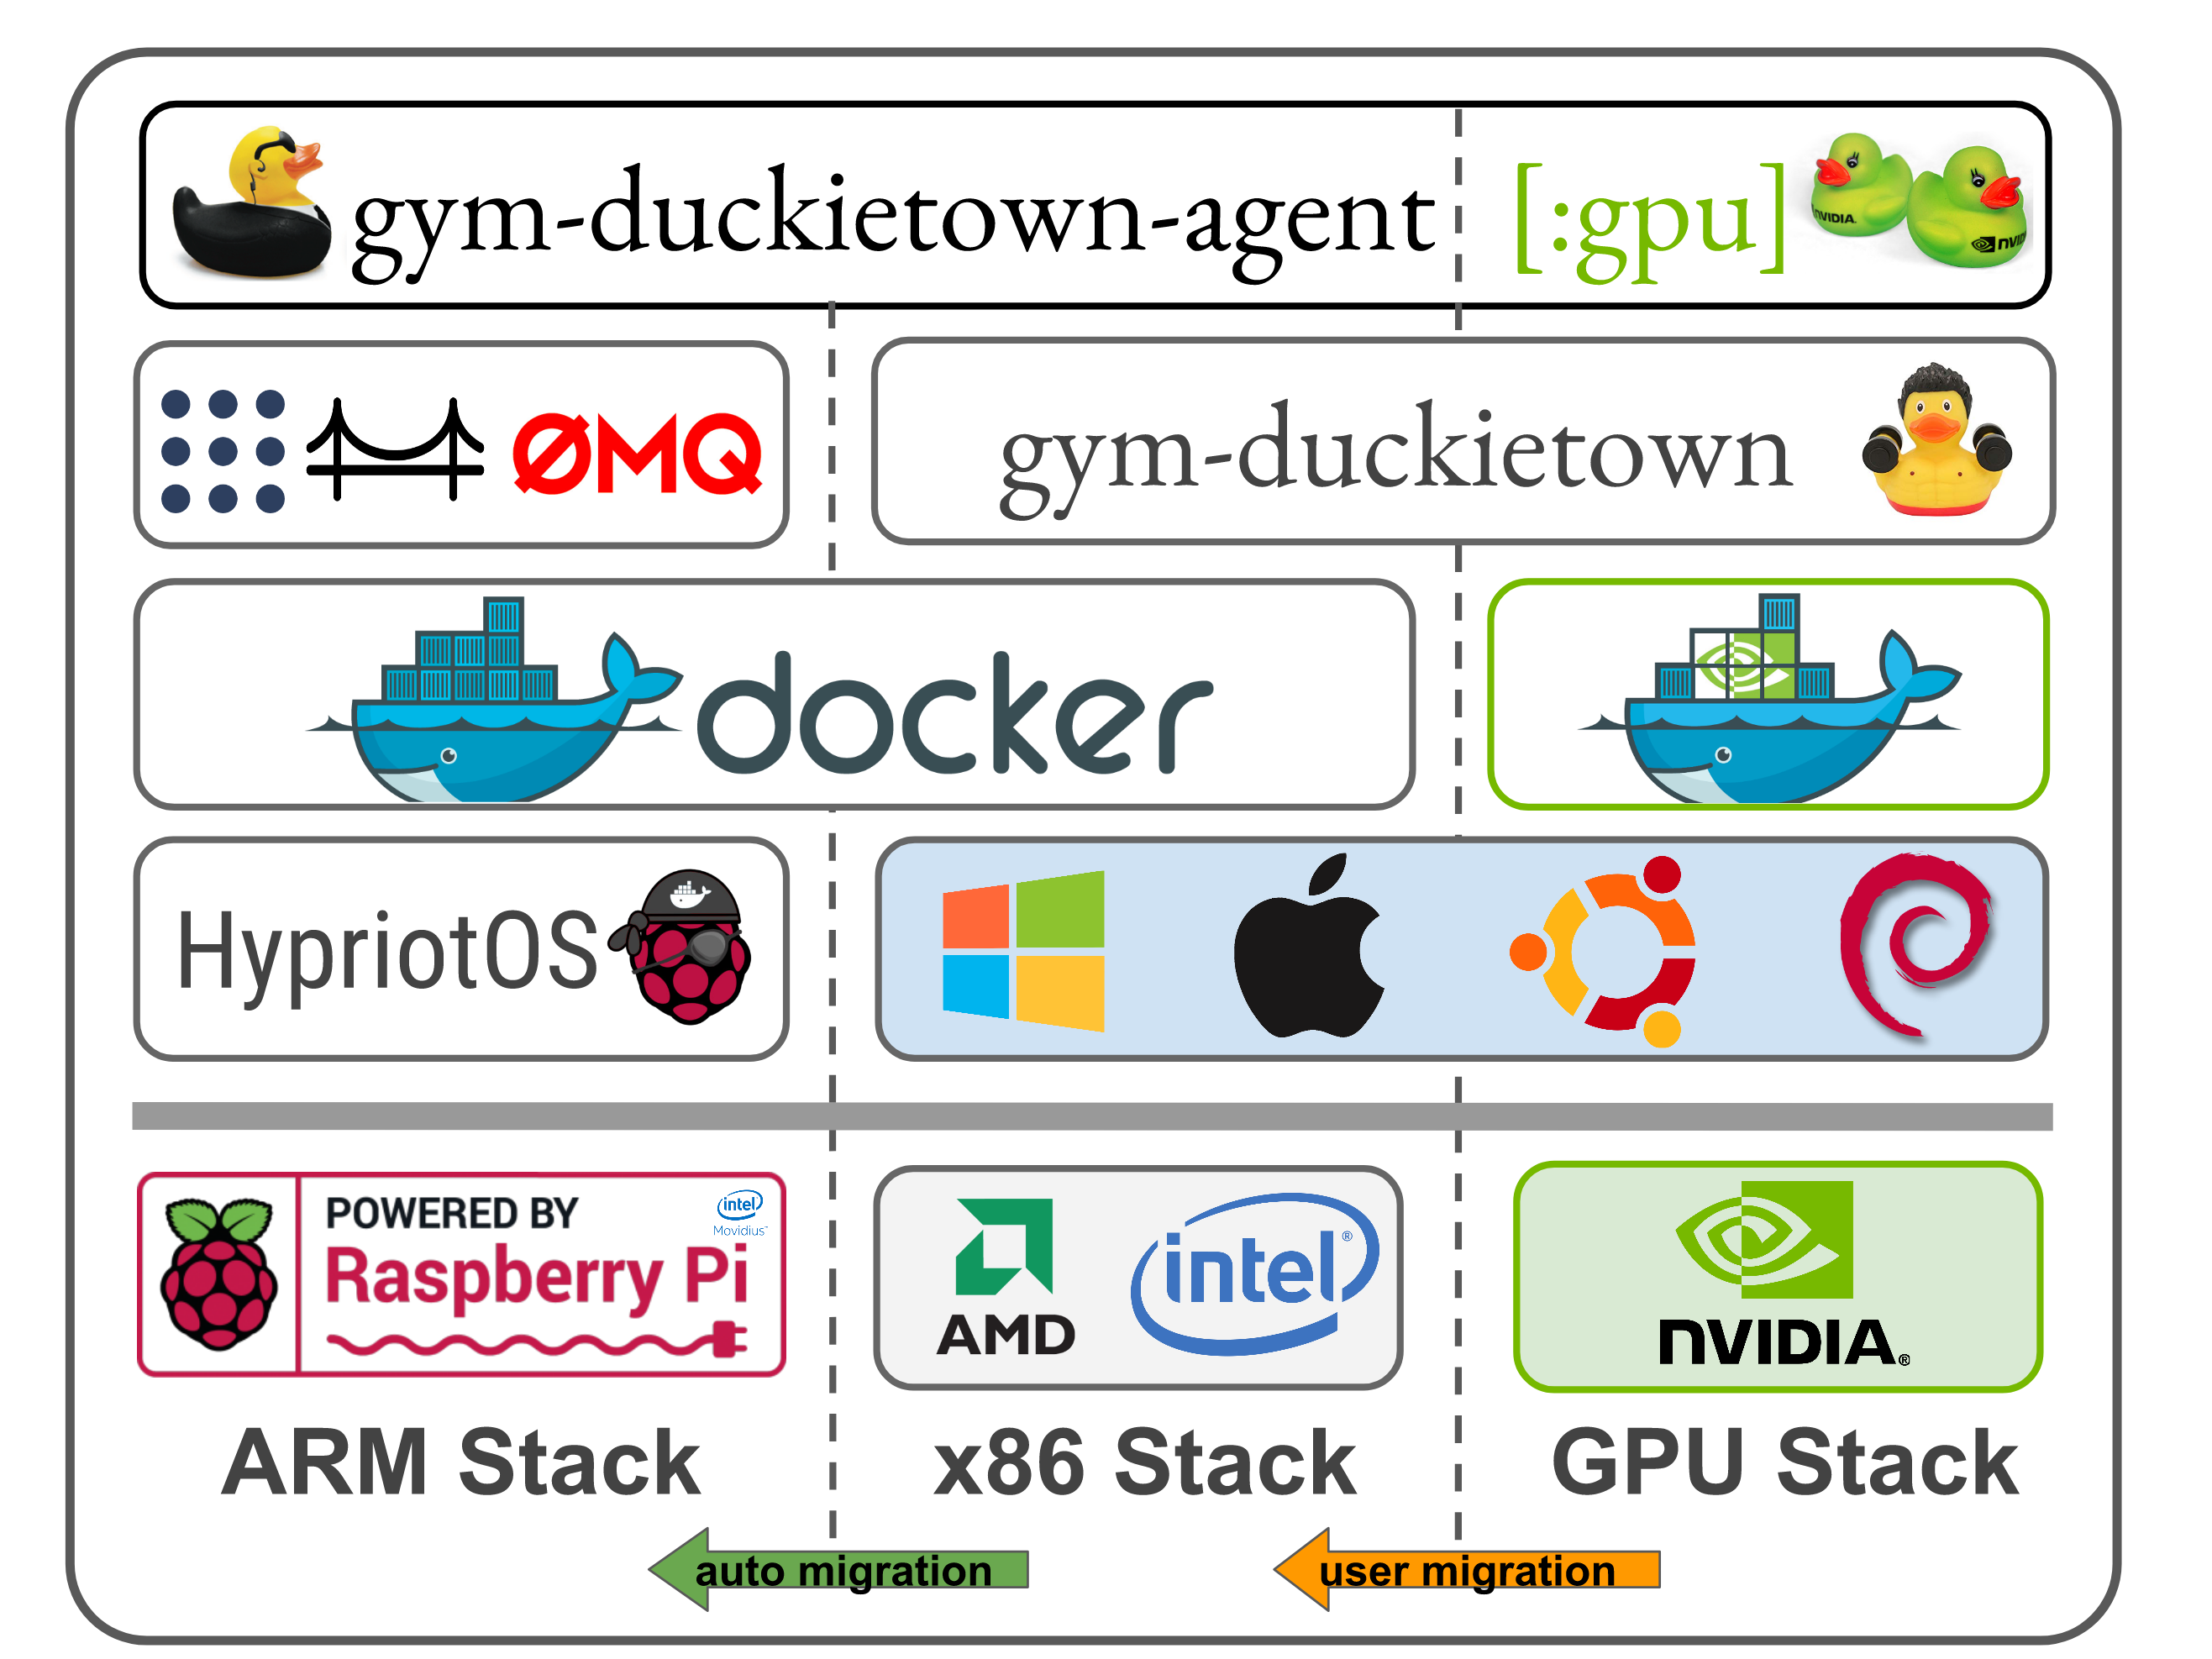
\includegraphics[width=0.45\textwidth]{docker_stack_2.png}
    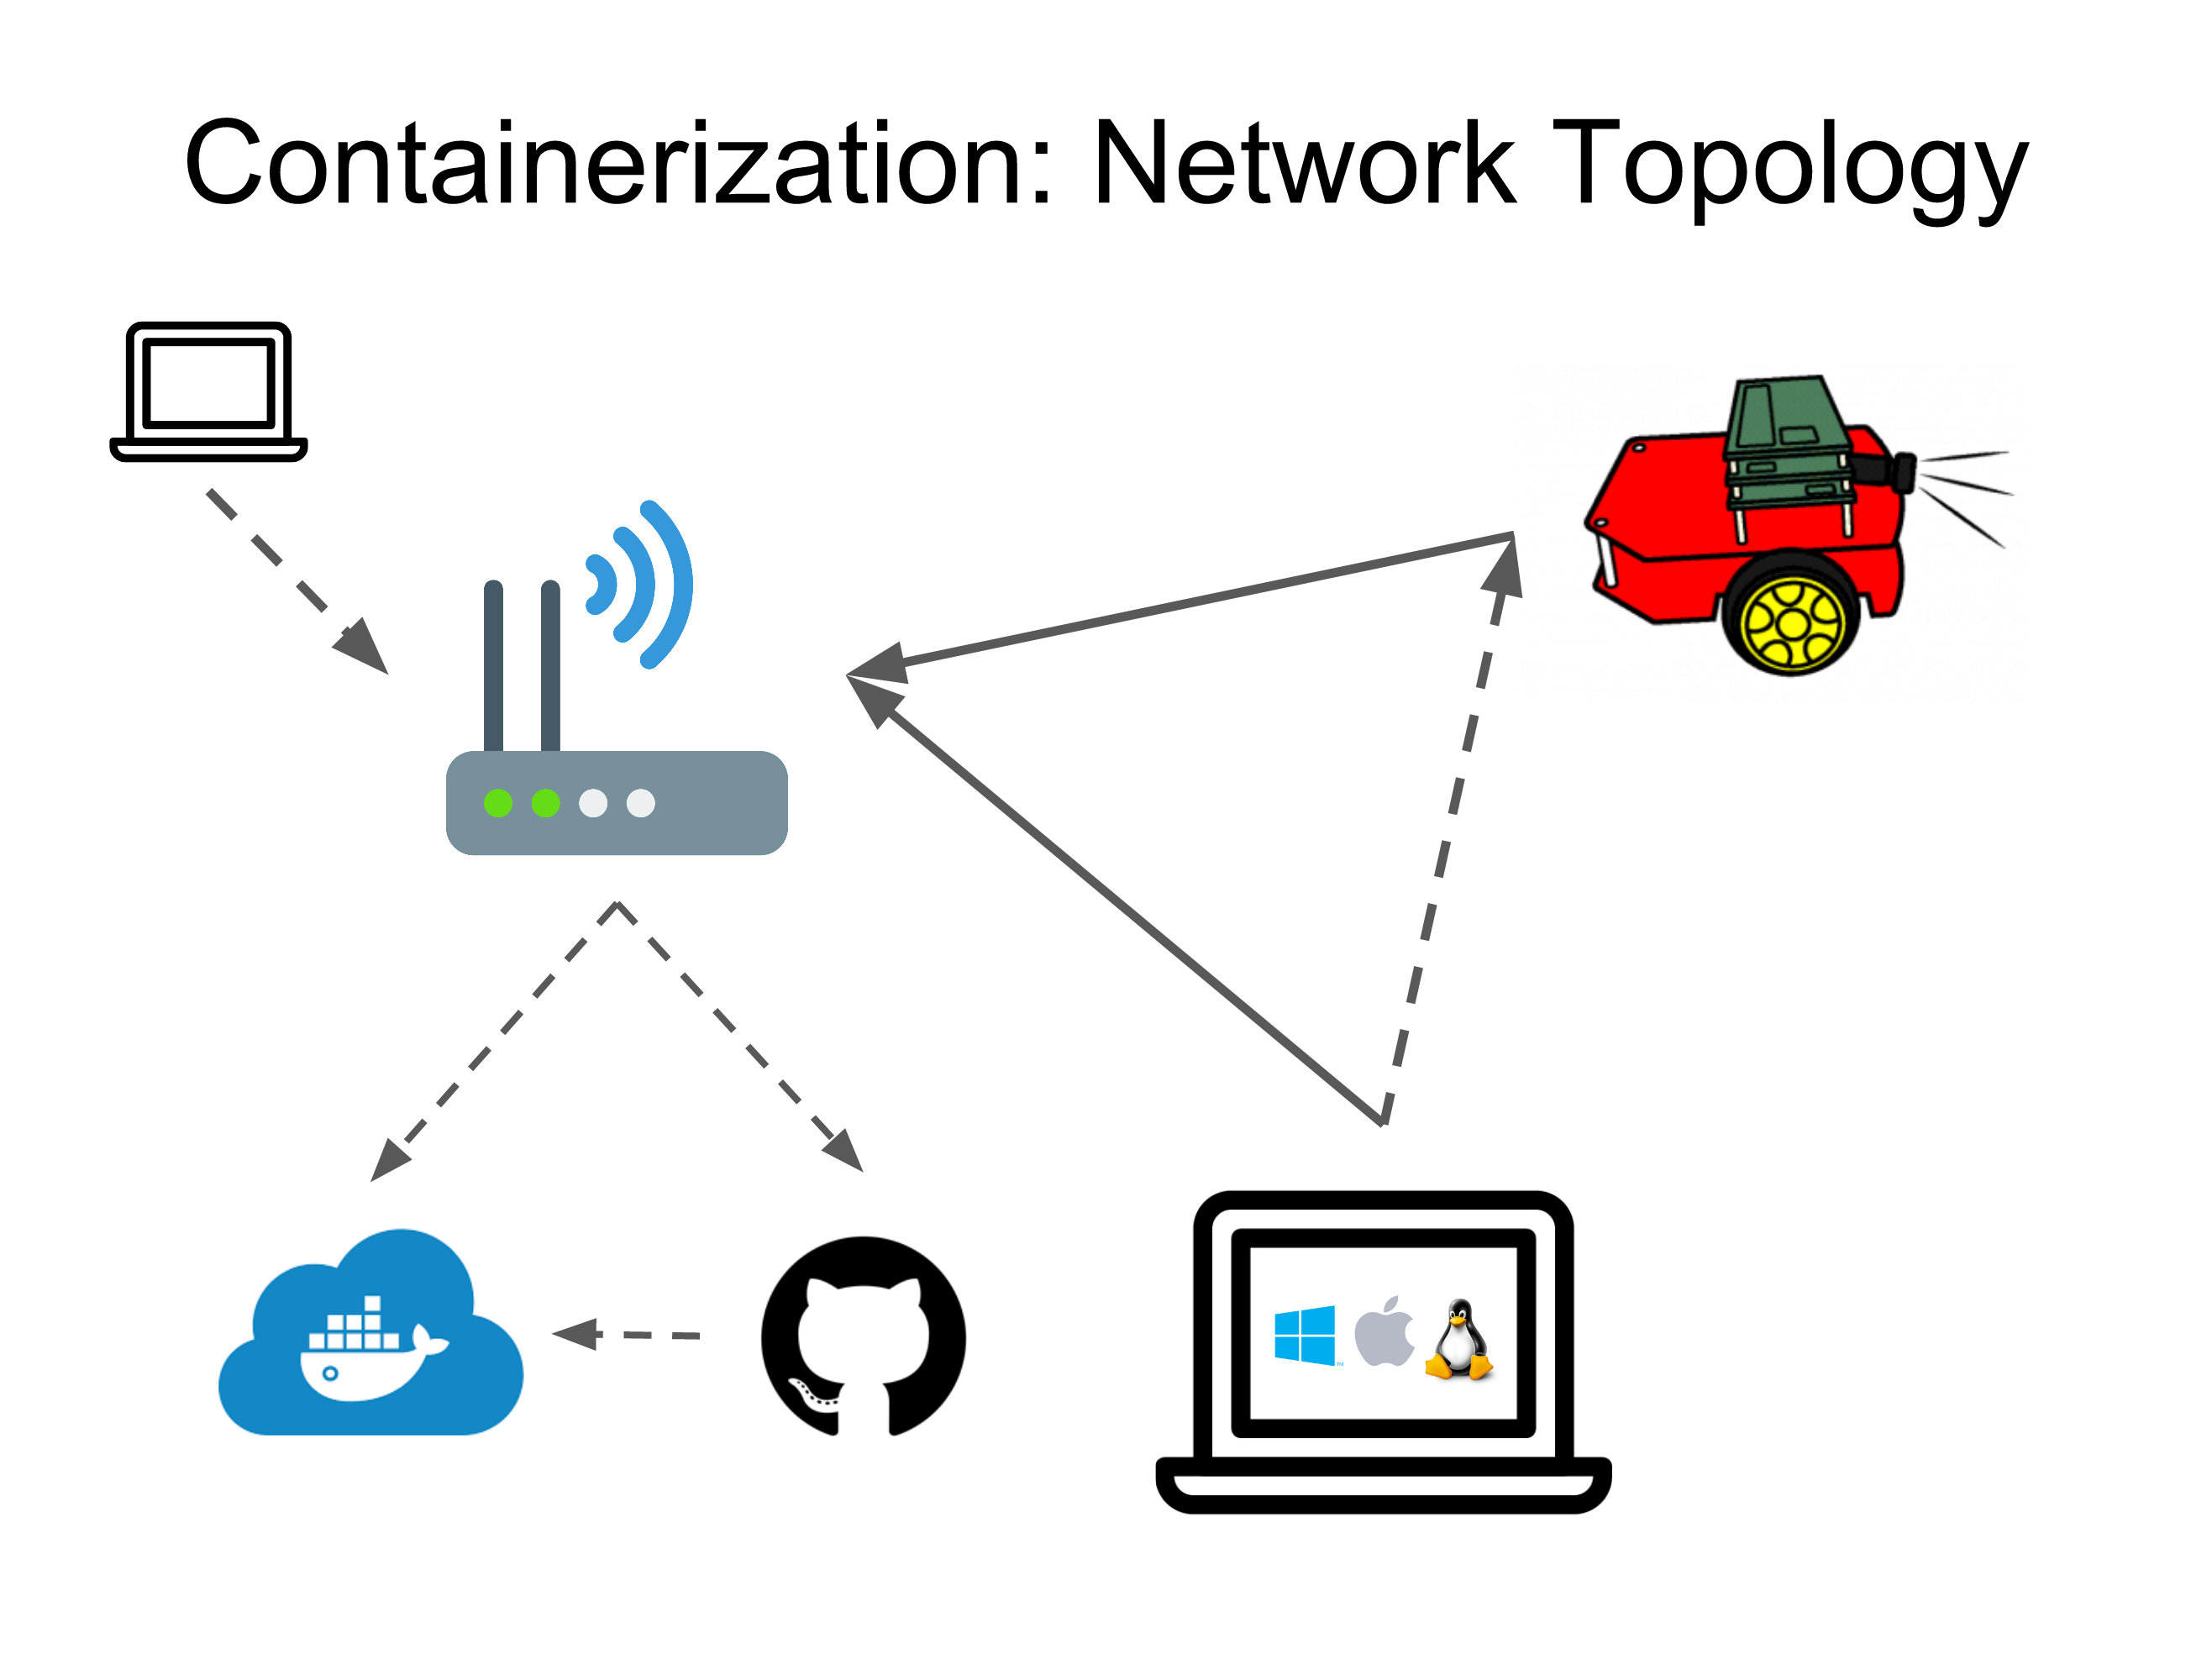
\includegraphics[width=0.35\textwidth]{network_infra.png}
    \caption{AI-DO container infrastructure. Left: The ROS stack targets two primary architectures, x86 and ARM. To simplify the build process, we only build ARM artifacts, and emulate ARM on x86. Right: Reinforcement learning stack. Build artifacts are typically trained on a GPU, and transferred to CPU for evaluation. Deep learning models, depending on their specific architecture, may be run on an ARM device using an Intel NCS.}
    \label{fig:docker}
\end{figure}

The Duckietown platform supports two primary instruction set architectures: x86 and ARM. To ensure the runtime compatibility of Duckietown packages, we cross-build using hardware virtualization to ensure build artifacts can be run on all target architectures. Runtime emulation of foreign artifacts is also possible, using a similar technique.\footnote{For more information, this technique is described in further depth at the following URL: \url{https://www.balena.io/blog/building-arm-containers-on-any-x86-machine-even-dockerhub/}.} For performance and simplicity, we only build ARM artifacts and use emulation where necessary (e.g., on x86 devices). On ARM-native, the base operating system is HypriotOS, a lightweight Debian distribution with built-in support for Docker. For both x86 and ARM-native, Docker is the underlying container platform upon which all user applications are run, inside a container.

Docker containers are sandboxed runtime environments that are portable, reproducible and version controlled. Each environment contains all the software dependencies necessary to run the packaged application(s), but remains isolated from the host OS and file system. Docker provides a mechanism to control the resources each container is permitted to access, and a separate Linux namespace for each container, isolating the network, users, and file system mounts. Unlike virtual machines, container-based virtualization like Docker only requires a lightweight kernel, and can support running many simultaneous containers with close to zero overhead. A single Raspberry Pi is capable of supporting hundreds of running containers.

While containerization considerably simplifies the process of building and deploying applications, it also introduces some additional complexity to the software development lifecycle. Docker, like most container platforms, uses a layered filesystem. This enables Docker to take an existing ``image'' and change it by installing new dependencies or modifying its functionality. Images may be based on a number of lower layers, which must periodically be updated. Care must be taken when designing the development pipeline to ensure that such updates do not silently break a subsequent layer as described earlier in Sec.~\ref{sec:dev-pipeline}.

One issue encountered is the matter of whether to package source code directly inside the container, or to store it separately. If source code is stored separately, a developer can use a shared volume on the host to build the artifacts. In this case, while build artifacts images may be standalone reproducible, they are not easily modified or inspected. The second method is to ship code directly inside the container, where any changes to the source code will trigger a subsequent rebuild, effectively tying the sources and the build artifacts together. Including source code alongside build artifacts has the benefit of improved reproducibility and diagnostics. If a competitor requires assistance, troubleshooting becomes much easier when the source code is directly accessible. However doing so adds some friction during development, which has caused competitors to struggle with environment setup. One solution is to store all sources on the local development environment and rebuild the Docker image periodically, copying sources into the image.

\section{Docker and ROS}

Prior work has explored the Dockerization of ROS containers~\cite{white2017ros-docker}. This work forms the basis for our own, which is extended specifically for the Duckietown platform~\cite{paull2017duckietown}.

\rare{\chapter{Case study: application for autonomous robotics}}

As a case study, we have implemented a mobile application using ROS, Docker, and Android, using the proposed toolchain.

\section{Design}

Designed with Hatchery.

\section{Implementation}

Implementation includes Kotlin$\nabla$

\section{Verification and validation}

Verified using property-based testing.

\section{Containerization}

Deployed and CI-tested using Docker.

\rare{\chapter{Conclusion}\label{ch:conclusion}}

\section{Future work}

\subsection{Requirements Engineering}

Often it is not possible, or desirable to summarize the performance of a complex system using a single variable. In multi-objective optimization, we have the notion of pareto-efficiency...

Traditional software engineering has followed a rigorous process model and testing methodology. This model has guided the development of traditional software engineering, intelligent systems will require a re-imagining of these ideas to build systems that adapts to its environment during operation. Intelligent systems are designed with objective functions, which are typically one- or low-dimensional metrics for evaluating the performance of the system. Most often, these take the form of a single criteria, such as an \textit{error} or \textit{loss} which can represent descriptive phenomena such as latency, safety, energy efficiency or any number of objective measures.

For example, in the design of a web based advertisement recommendation system, we can optimize for various objectives such as click rate, engagement, sales conversion. So long as we can measure these parameters, with today's powerful function approximators, we can optimize for any singly criterion or combination thereof. Much of the work involved in machine learning is to find representations which are amenable to learning, and preventing unintended consequences. For example, by optimizing for click rate, we create an artificial market for click bots. Similarly, in self driving cars, we often want to optimize for passenger safety. However by doing so naively, we create a vehicle that never moves, or always yields to nearby vehicles.

When building intelligent system developers must first ask, what are the requirements of the system? This process is often the most troublesome part, because the requirements must not be fuzzy specifications like traditional software engineering, but precise, programmable directives. "I would like the system to be fast," is not sufficiently precise. These kinds of requirements must be translated into statistical loss functions, so we must be very precise about how we specify our requirements. If we simply say, "The system must produce a valid response as quickly as possible, in less than 100ms," is better, but leaves open the possibility of returning an empty response.

In traditional software engineering, it is reasonable to assume the people who are implementing the system have some implicit knowledge and are generally well-intentioned human beings working towards the same goal. When building an intelligent system, a more reasonable assumption is that the entity implementing our requirements is a naive but powerful genie, and possibly an adversary. If we are to give it an optimization metric, it will take every conceivable shortcut to achieve that metric. If we are not careful about requirements engineering, this entity can produce a system that does not work, or has unintended consequences.

In the strictest sense, designing a good set of requirements is indistinguishable from implementing the system. With the right language abstractions (e.g.\ declarative programming), requirements and implementation can be the same thing. These ideas have been explored in recent decades with languages like SQL and Prolog. While these are toy systems, neural networks can express much larger classes of functions than traditional software engineering.

\subsection{Continuous Delivery and Continual Learning}

An overall trend in software and systems engineering is the transition away from long development cycles towards continuous integration and deployment. Development teams in the industry are encouraged to iterate in a series of short sprints between feature development and deployment. In some cases, software is shipped to users on a nightly basis, with automated testing and deployment. Similarly, intelligent systems have a need to continuously adapt to their environment, and will change their code on an even shorter basis.

Incremental updates will grow increasingly smaller, until the program starts to alter itself after every input it processes.

We need tools to more effectively harness the stochasticity of these learning systems.

\subsection{Developers, Operations, and the DevOps toolchain}

Software engineers have begun to realize the value of bespoke tools that facilitate the process of shipping software, in addition to the software itself.

Teams building software are cybernetic systems, and require meta-programs for building code and organizational processes which enable them to ship code more efficiently.

\bibliography{thesis}
\bibliographystyle{plain}
\end{document}